%TEX root = ../dissertation.tex

\chapter{Pulsarcast}
\label{chapter:pulsarcast}

Pulsarcast is a peer to peer, pub-sub, topic-based system focused on
reliability, eventual delivery guarantees, and data persistence. We seek this
while not fully compromising the scalability given by the decentralised nature
of our architecture. Looking through our related work, it became clear that few
fully decentralised solutions exist that try to provide this kind of
guarantees. Yet, if we carefully look at the most popular and widely adopted
centralised pub-sub solutions, it is clear that most of them heavily rely and
depend upon these same guarantees. 

We opted for the more straightforward topic-based subscription model given
that, in our view, a well structured and implemented topic-based model is more
than enough for a significant percentage of our use cases. In the end, we
compromise a bit of the expressiveness of the system in order to avoid bringing
more complexity in, something we believe will pay off.

We divided this chapter as follows. We start by covering the use case of our
system in Section \ref{use-case}, where we will introduce some of our broader
architectural decisions. Next, we will move to Section \ref{data-structures}
where we will deep dive into Pulsarcast's data structure model and how it is
distributed across the network. Afterwards, we will look into one of the most
critical parts of our architecture in Section
\ref{subscription-management-event-dissemination} where, based on the covered
related work and the taxonomy we defined, we present the algorithms and
mechanisms used for managing the subscriptions and event dissemination. We
finish this chapter by looking into the \acrshort{rpc} messages that power the
Pulsarcast API in Section \ref{rpc-message}

\section{Use Case}\label{use-case}

Pulsarcast is a fully decentralised solution, which means that each node plays
a crucial part in fulfilling the system's purpose, delivering events and
ensuring their dissemination. Conceptually speaking, Pulsarcast provides four
methods for clients and applications to interact with the system, create a
topic, subscribe to a topic, unsubscribe from a topic and publish an event in a
topic. From a broader perspective, Pulsarcast relies on two overlays to fulfil
its needs. Kadmelia \acrshort{dht}, already employed by IPFS and used by
Pulsarcast for peer discovery, content discovery and to bootstrap our other
overlay, the Pulsarcast own overlay. The Pulsarcast overlay is actually a set of
different overlays or, as we call it, dissemination trees.  These trees are on
a per topic basis and are the critical factor in the way we disseminate
information across our decentralised network.  Figure
\ref{fig:pulsarcast-overlays} illustrates the multiple overlays in action.

\begin{figure}[hb!]
  \centering
  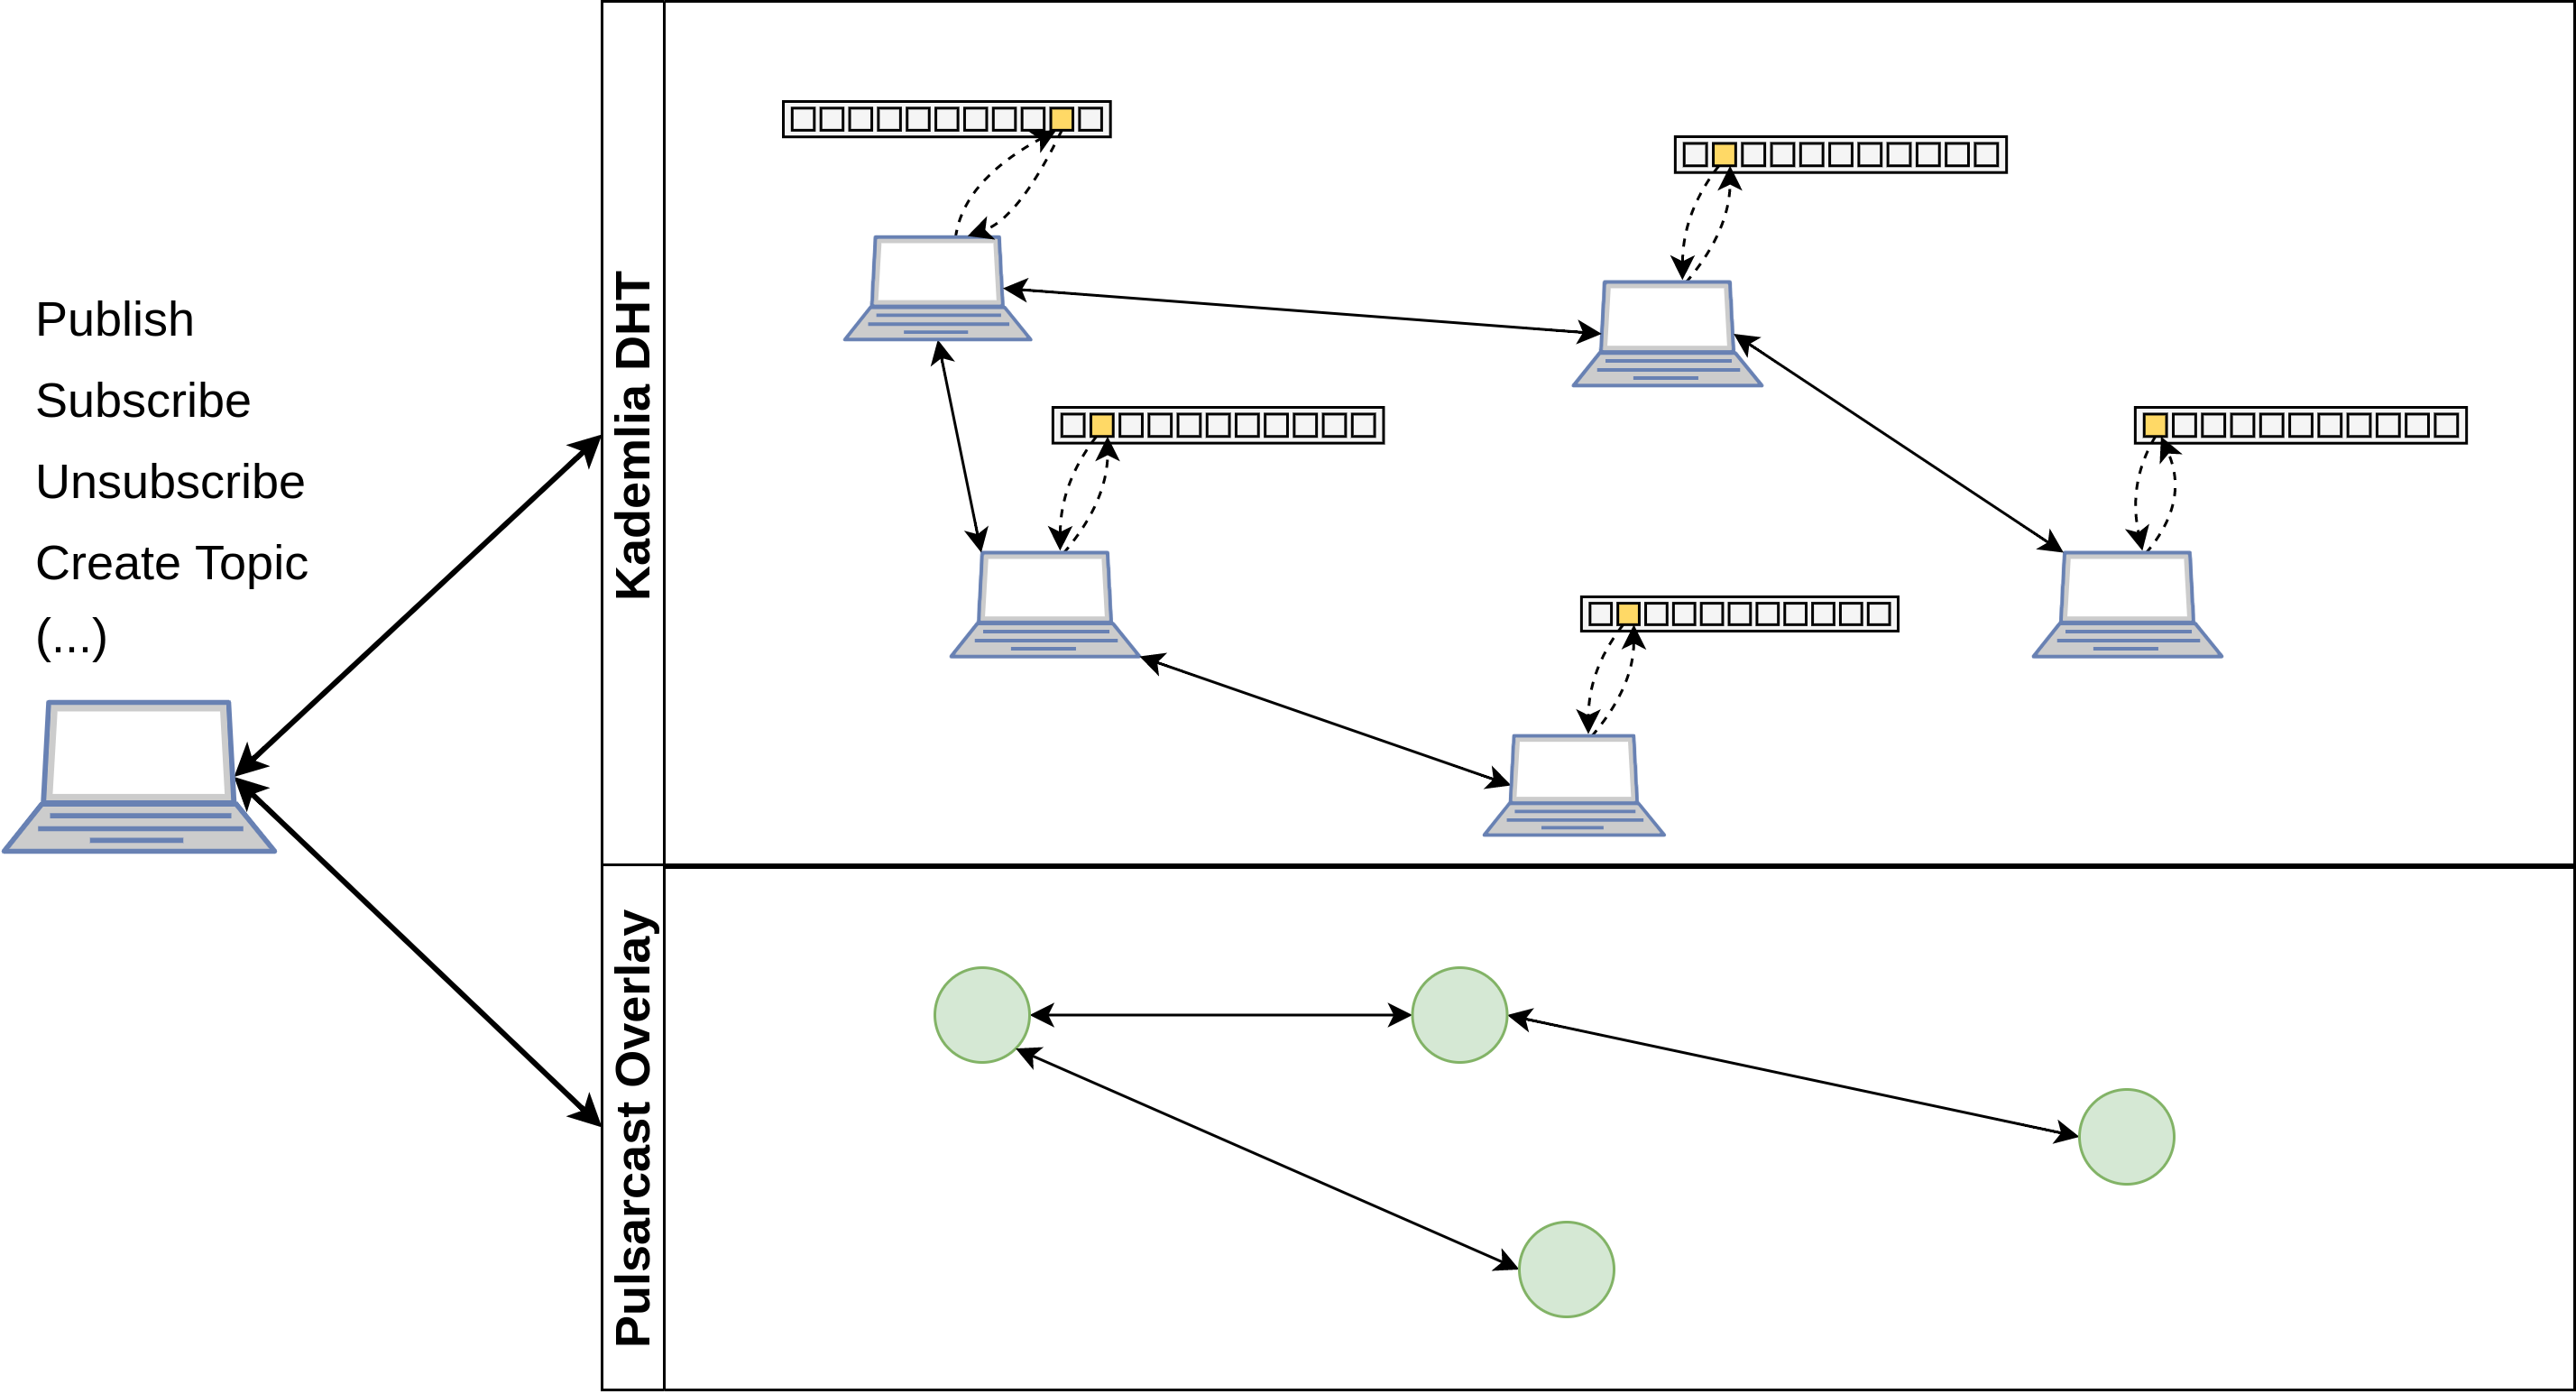
\includegraphics[width=0.95\textwidth]{img/pulsarcast-overlays.png}
  \caption{Representation of the Pulsarcast overlays}
  \label{fig:pulsarcast-overlays}
\end{figure}

The subscription model followed by Pulsarcast is a topic based one, but still
allowing for some expressiveness through the usage of sub-topics to enable more
complex structures. When a peer publishes an event or creates a new topic a set
of the overlays described is used accordingly. For Pulsarcast, both of these
actions, happen to take a similar course. That is because the system views
these pieces of information (or descriptors as we call it) as fairly similar,
given their importance. Figures \ref{fig:pulsarcast-descriptor-creation} and
\ref{fig:pulsarcast-descriptor-query} provide an overview of how the flows for
creating this information and for accessing it look like.

\begin{figure}[hb!]
  \centering
  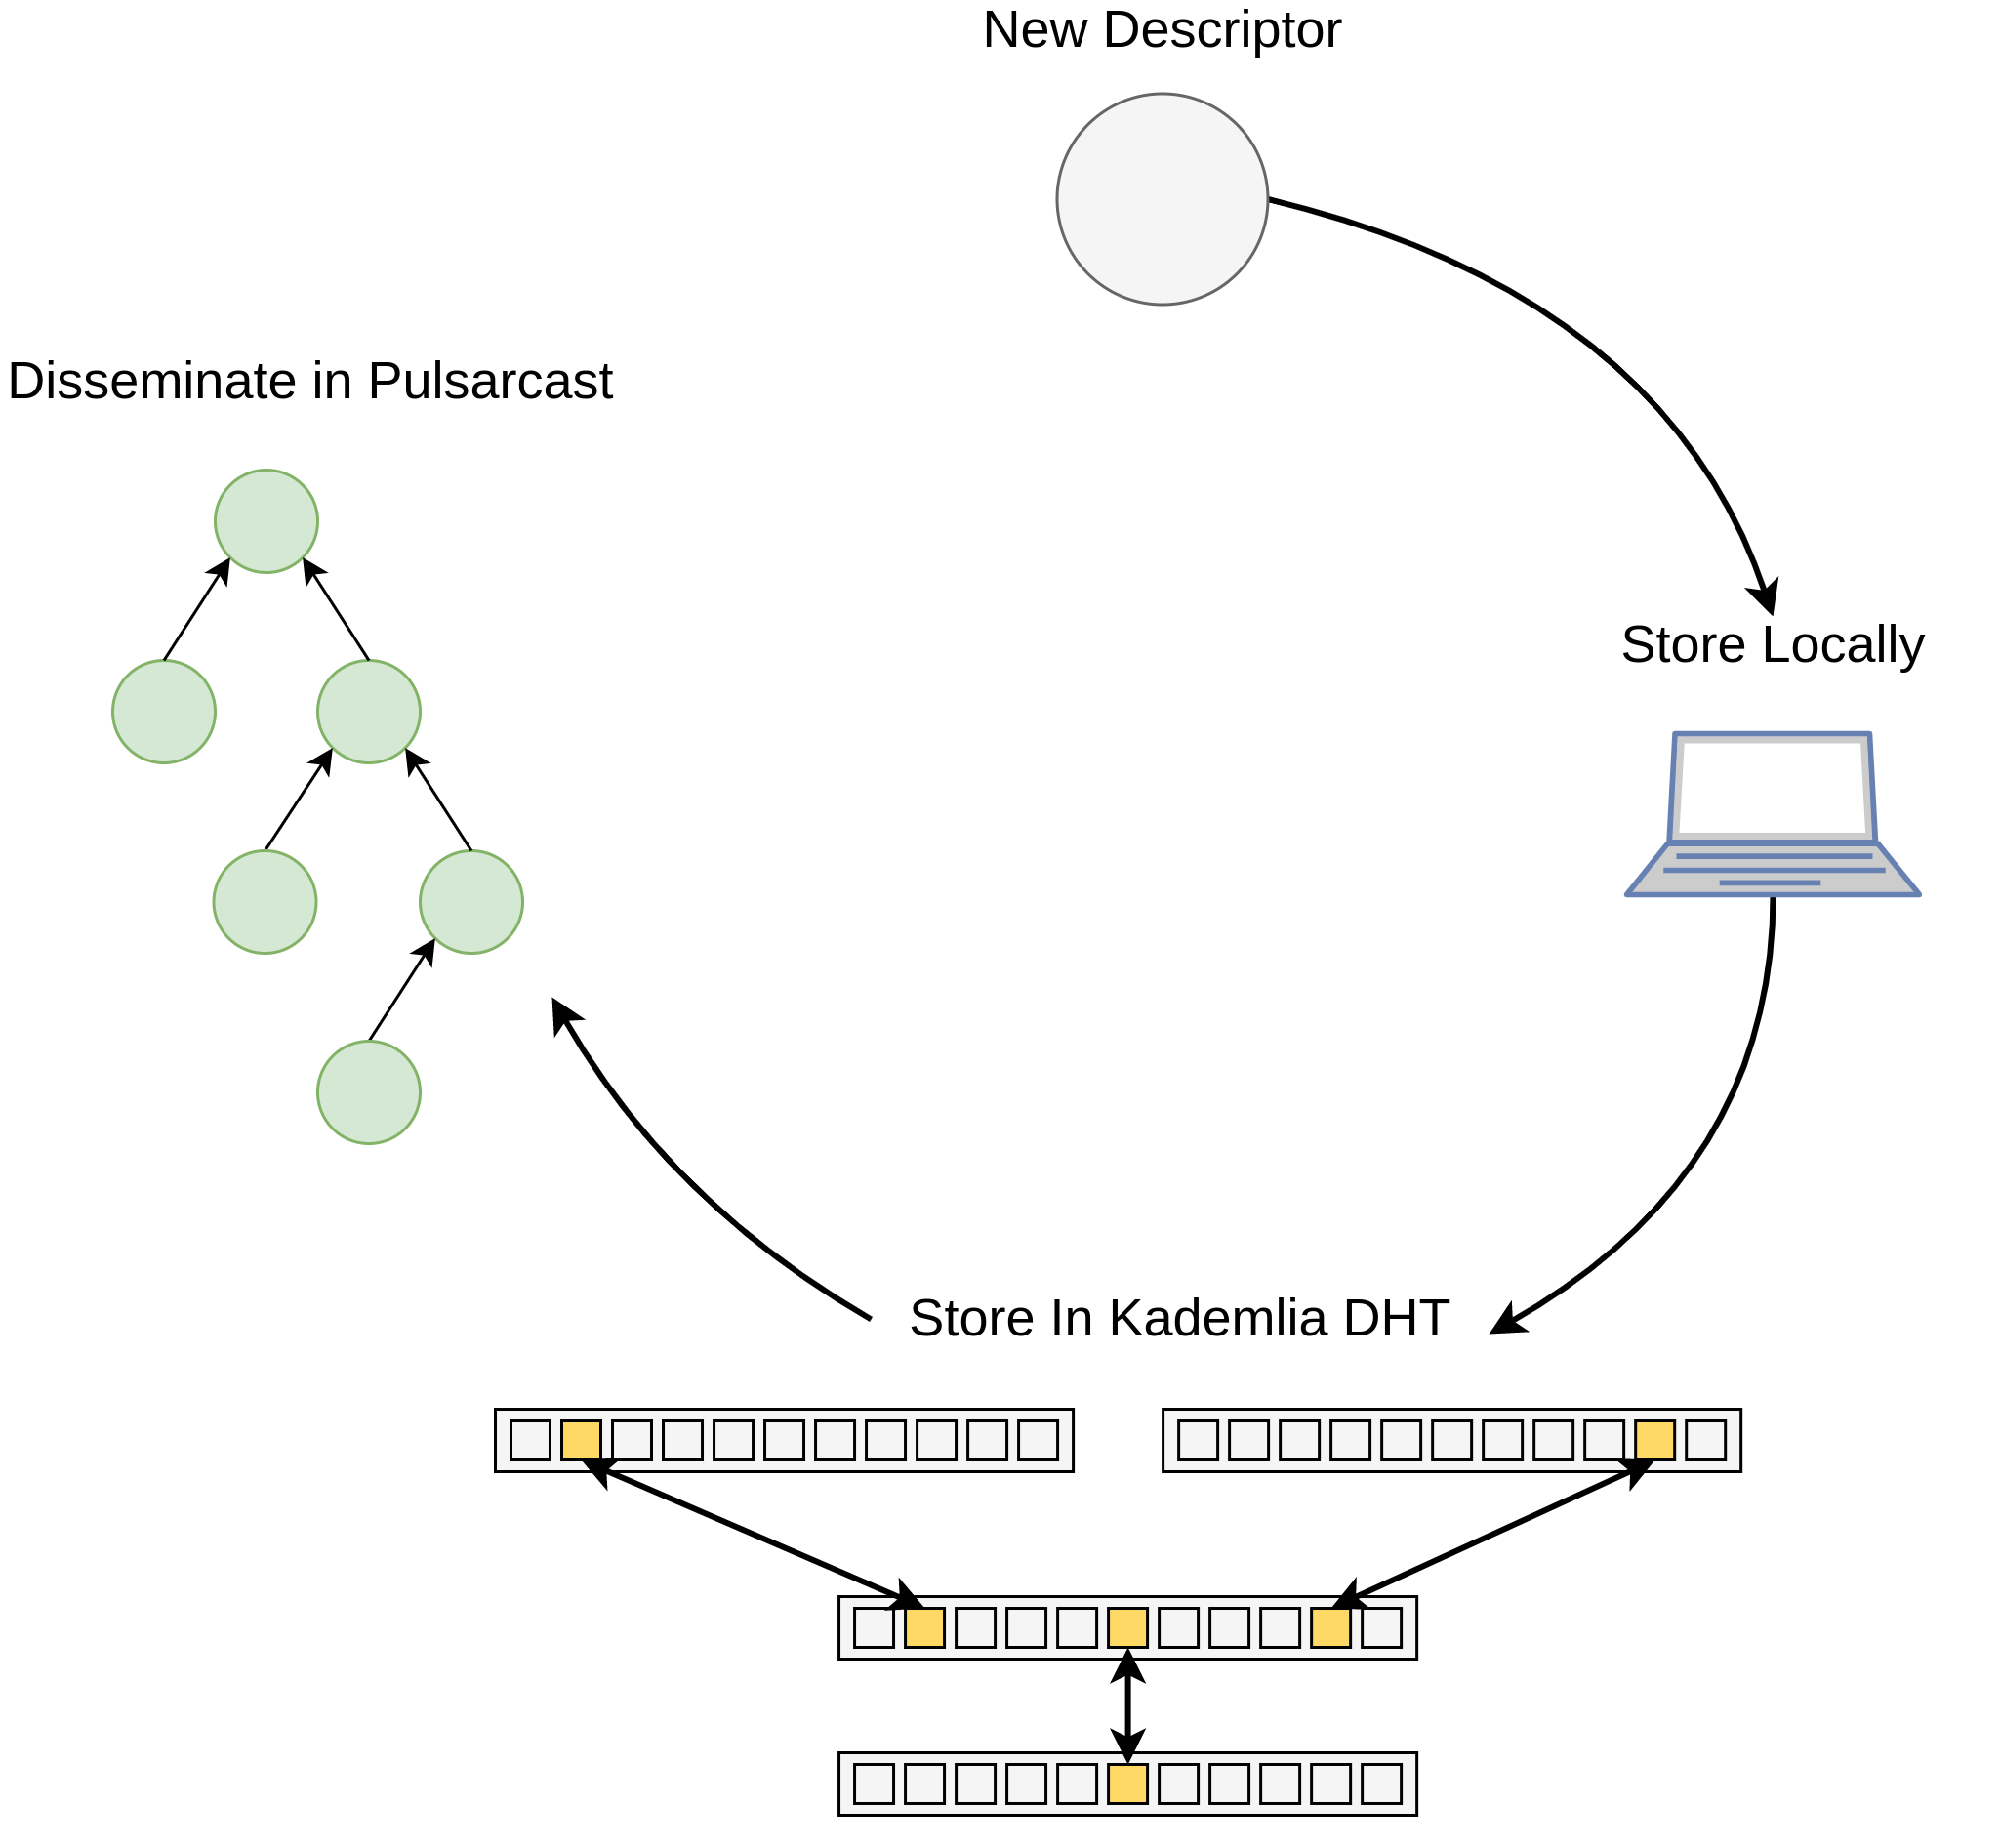
\includegraphics[width=0.7\textwidth]{img/pulsarcast-descriptor-creation.png}
  \caption{Flow for creating a new Topic/Event descriptor}
  \label{fig:pulsarcast-descriptor-creation}
\end{figure}

\begin{figure}[tb!]
  \centering
  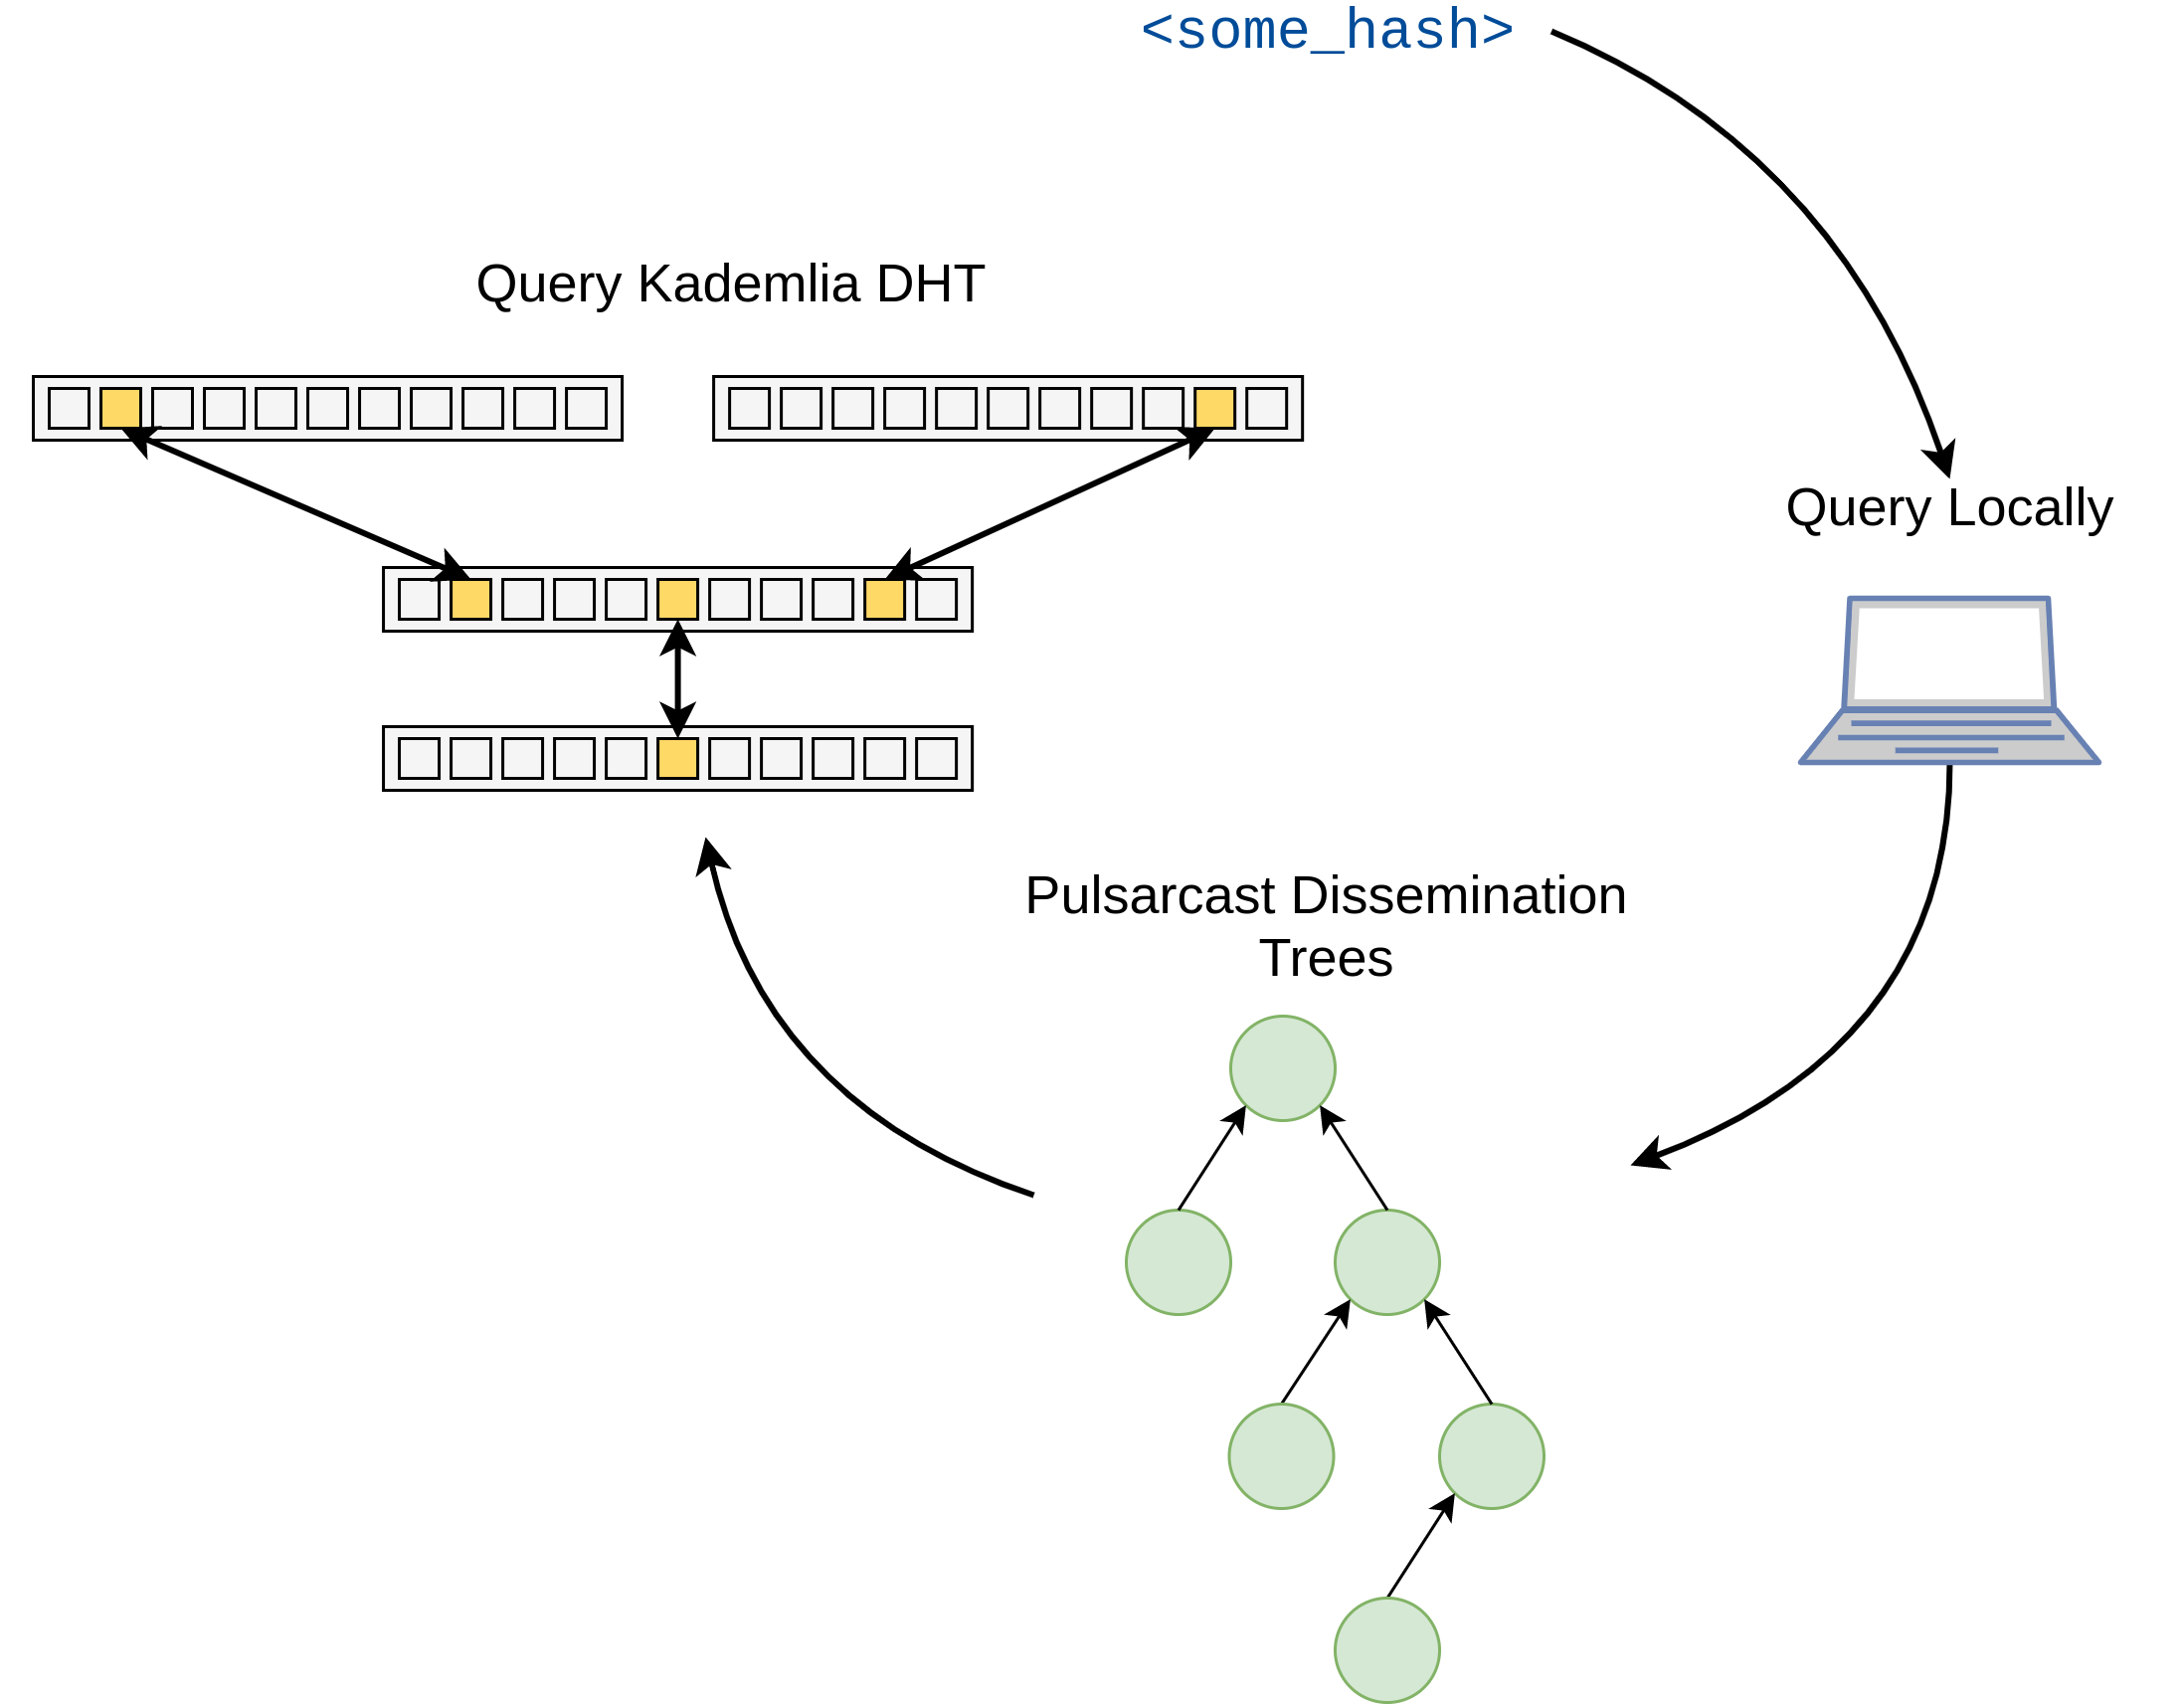
\includegraphics[width=0.7\textwidth]{img/pulsarcast-descriptor-query.png}
  \caption{Flow for querying a Topic/Event descriptor}
  \label{fig:pulsarcast-descriptor-query}
\end{figure}

Pulsarcast's goal is to give users and any applications built on top of it the
reassurance that events reach their destination and that they can rebuild as
much of the event or topic history as they see fit. As such, we doubled our
efforts to persist and propagate data. Every topic and event is stored in the
Kadmelia \acrshort{dht} before being forwarded through the topic dissemination
trees.  This ensures the data is persisted by a set of nodes (that might even
be extraneous to the topic at hand) and anyone is later able to fetch the data
using only the \acrshort{dht} if they want to. Afterwards, we forward the data
through the appropriate dissemination trees previously built (we will cover
this process in Section \ref{subscription-management-event-dissemination}).
Currently, every node participating in the data transmission through the
dissemination tree stores it indefinitely, although it is something due to
being changed in a later revision of our protocol (e.g. by means of predefined
global or topic-specific temporal time-out, or by a special message per topic
flushing all past events up to a specific one). On the other hand, when someone
wants to fetch a piece of data (a topic or an event) it starts by performing a
local search in the system, it might have been something that the node has run
through when forwarding events across their dissemination trees. If this fails,
though, a query to the \acrshort{dht} is in order.

\section{Data Structures}\label{data-structures}

Pulsarcast has a set of two fundamental data structures to which we refer to as
\textbf{event} and \textbf{topic descriptors}. To help us represent this data,
we rely on a concept already introduced in our related work, the Merkle
\acrshort{dag}.

\subsection{Content-Addressability}\label{subsec:content-addressability}

All of our data structures are immutable, content addressable and linked
together to form a \acrlong{dag} (Merkle \acrshort{dag}). Events link both to
their respective topic descriptor and a past event in that topic. Topics, on
the other hand, link to their sub-topics (if any) and a previous version of
themselves.  Figure \ref{fig:pulsarcast-dag} provides a broader picture of how
it all fits together. Immutability and content-addressability give us
verifiability. Consequently, the assurance that the state of our distributed
system is the same no matter where we are accessing it from or who is viewing
it. It also allows us to build a notion of history which plays nicely into a
pub-sub scenario. Through these links and the mechanisms described in the
previous section, users and applications are free to rebuild their topic and
event history to any point they wish. Be that because they were not part of the
network at the time or because they missed out due to some system or network
failure, acting as a NACK (not acknowledged) for relevant events.

\begin{figure}[hb!]
  \centering
  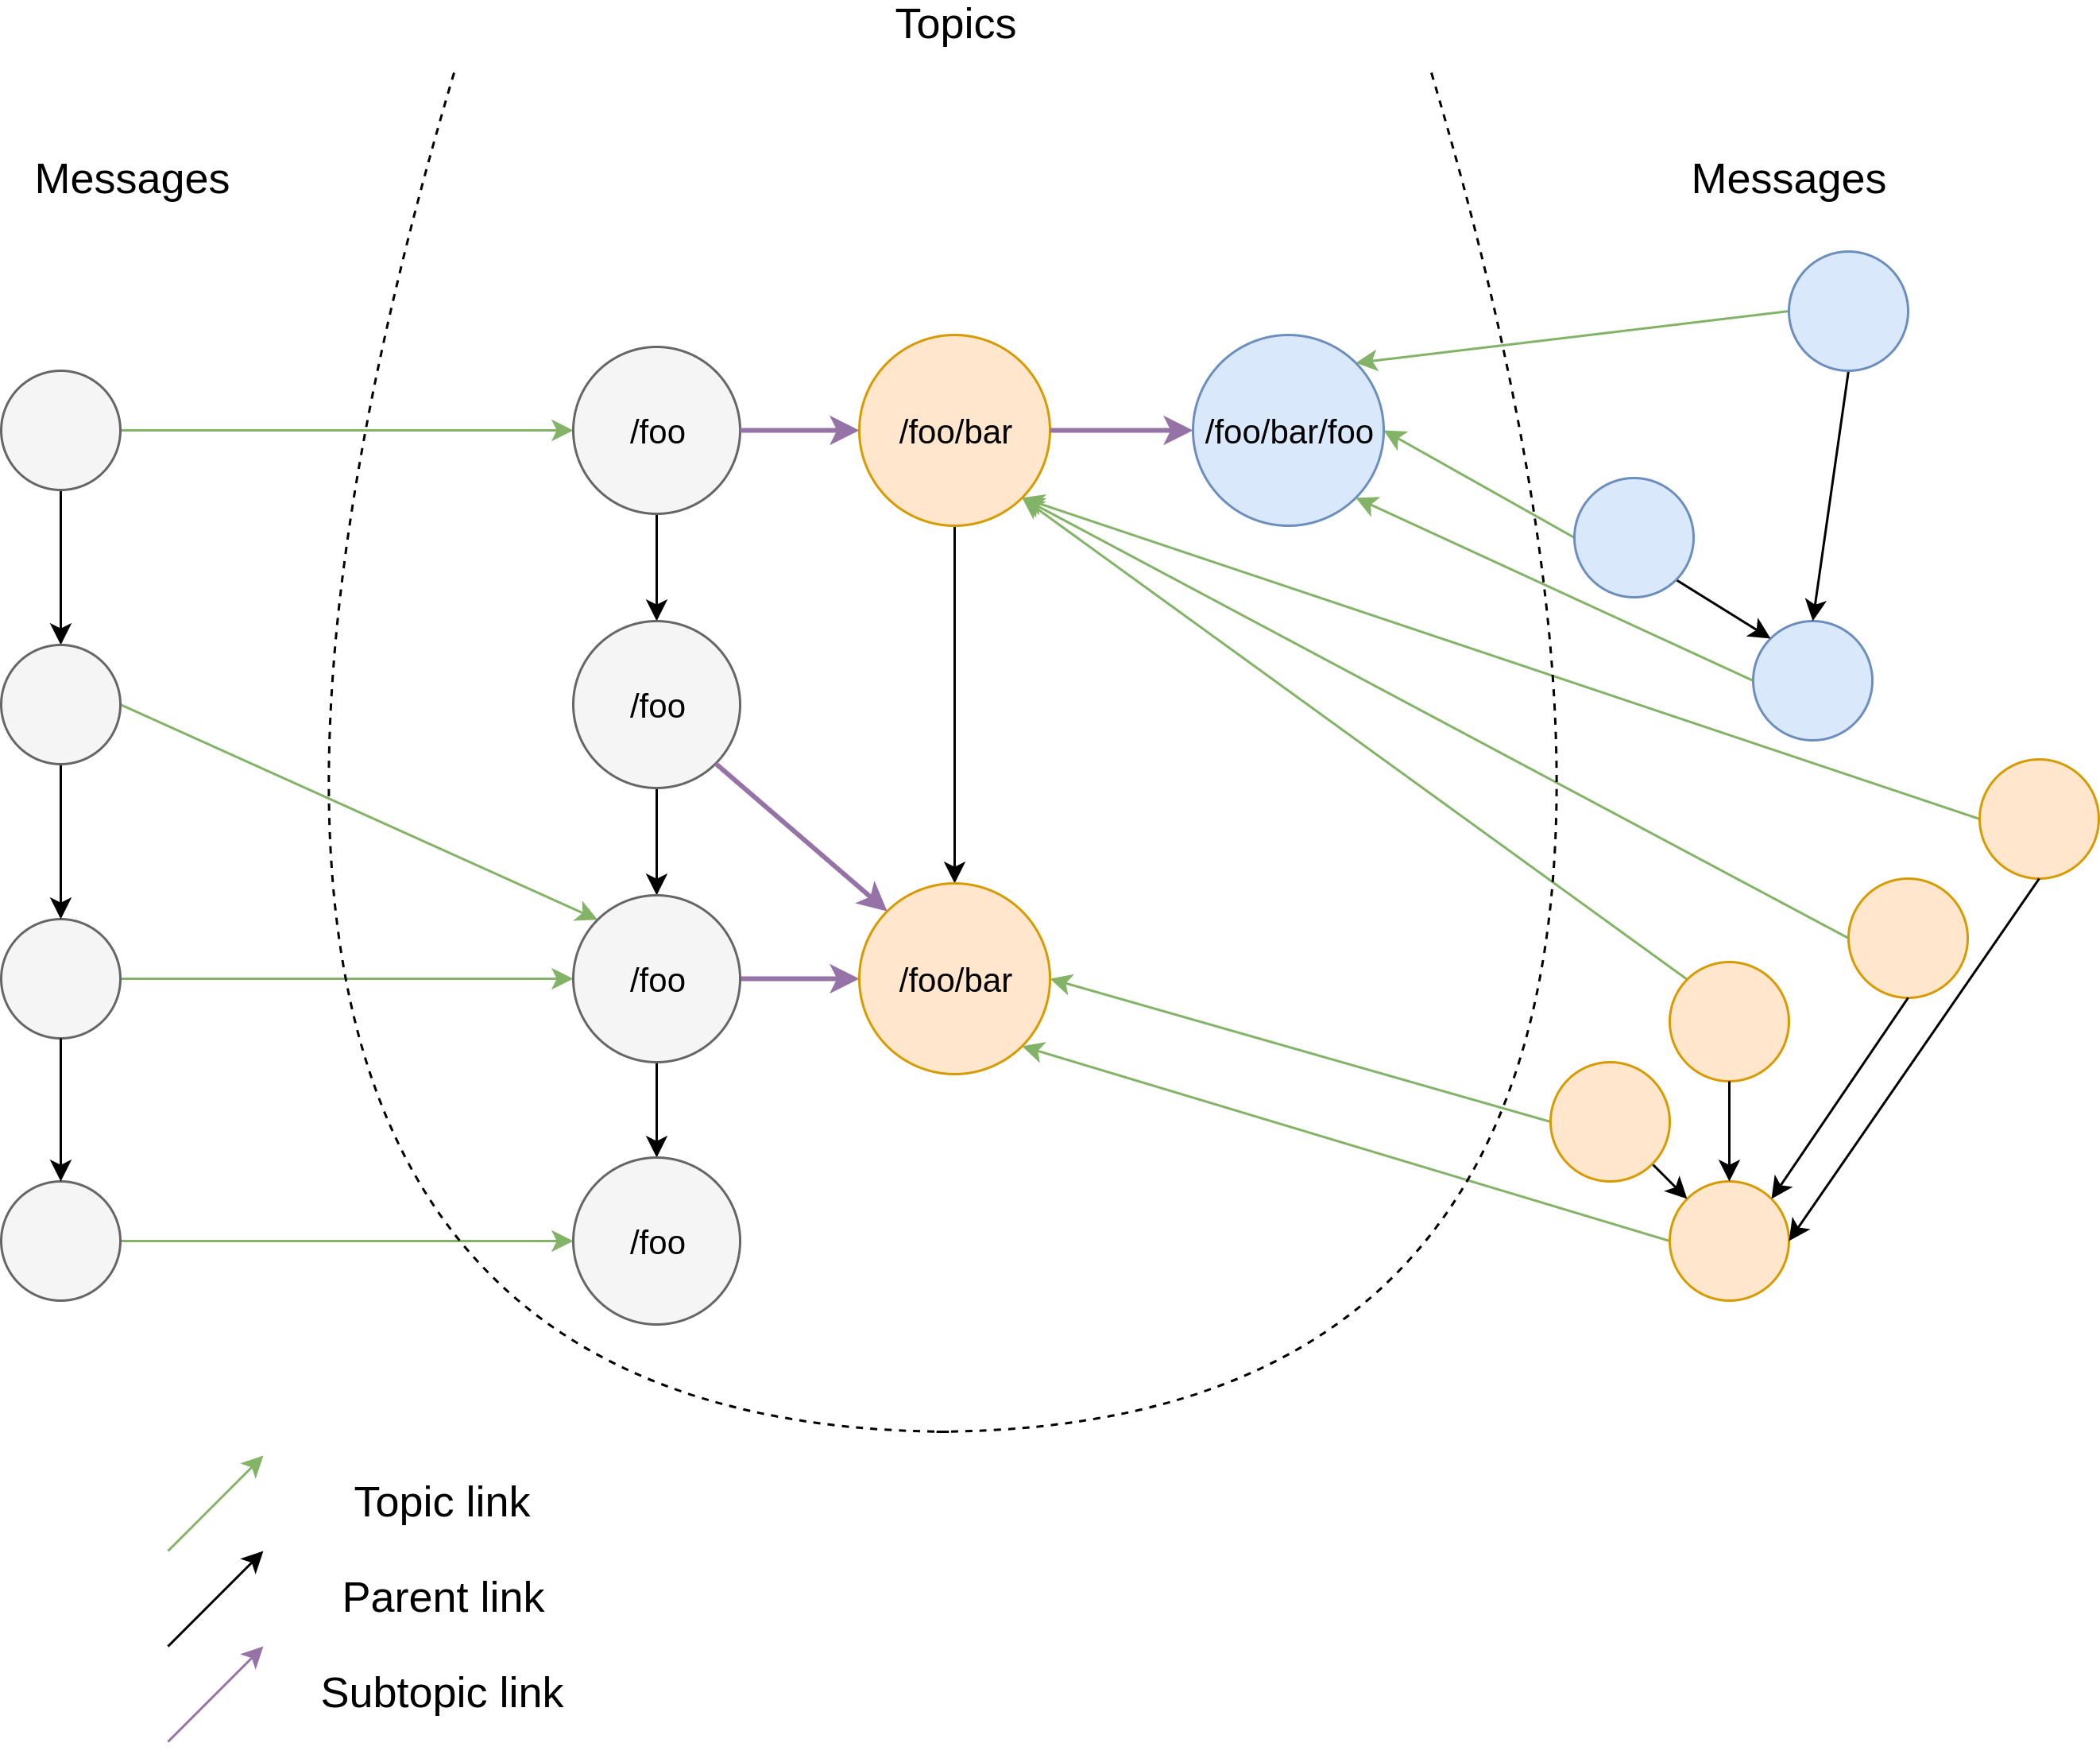
\includegraphics[width=0.95\textwidth]{img/pulsarcast-dag.png}
  \caption{Representation of the Pulsarcast \acrshort{dag}}
  \label{fig:pulsarcast-dag}
\end{figure}

Given we are discussing addressability and linking between content, the
representation used for our identifiers is an important part of our system
specification. That was one of the main reasons for us to borrow inspiration
from systems like \acrshort{ipfs} and decided to use \emph{CIDs} (Content
Identifiers)~\footnote{\url{https://github.com/multiformats/cid}}.  A CID is a
self-describing content-addressed identifier. It uses cryptographic hashes to
achieve content addressing and is powered by
\emph{multihash}~\footnote{\url{https://github.com/multiformats/multihash}}.
Multihash is a convention for representing the output of many different
cryptographic hash functions in a compact, deterministic encoding that is
accommodating of future change. This is because multihash encodes the type of
hash function used to produce the output. All of the relevant identifiers in
our system are CIDs. This includes node identifiers as well as the identifiers
for both event descriptors and topic descriptors themselves (given they are the
hash of its content). The descriptors contain a set of relevant metadata as
well as the actual information that they refer to. The following JSON like
Listings \ref{topic-descriptor} and \ref{event-descriptor} provide an accurate
description of the schema and format of our data structures. We will cover some
of the properties.

% \noindent\begin{minipage}{\textwidth}
% \vspace{8pt}
\begin{lstlisting}[float, language=JSON,caption={Topic descriptor schema in a JSON based format},label={topic-descriptor}]
{
  "name": <string>,
  "author": <peer-id>,
  "parent": {                     //The parent link for this topic
    "/": <topic-id>
  },
  "#": {                          //Sub topic links
		"meta": {												//Meta topic
			"/": "zdpuAkx9dPaPve3H9ezrtSipCSUhBCGt53EENDv8PrfZNmRnk"
		},
    <topic-name>: {
      "/": <topic-id>
    },
    ...
  },
  "metadata": {
    "created": <date-iso-8601>,
    "protocolVersion": <string>,  //Pulsarcast protocol version
    "allowedPublishers": {        //If enabled, whitelist of allowed publishers
      "enabled": <boolean>,
      "peers": [ <peer-id> ]
    },
    "requestToPublish": {         //Enable request to publish
      "enabled": <boolean>,
      "peers": [ <peer-id> ]      //Optional whitelist able to request
    },
    "eventLinking": <string>,     //One of: LAST_SEEN, CUSTOM
  }
}
\end{lstlisting}
% \vspace{8pt}
% \end{minipage}

% \noindent\begin{minipage}{\textwidth}
% \vspace{8pt}
\begin{lstlisting}[float, language=JSON,caption={Event descriptor schema in a JSON based format},label={event-descriptor}]
{
  "name": <string>,
  "publisher": <peer-id>,         //Peer who published the event
  "author": <peer-id>,            //Author of the event
  "parent": {                     //The parent link for this event
    "/": <topic-id>
  },
  "topic": {
    "/": <topic-id>
  },
  "payload": <binary-data>
  "metadata": {
    "created": <date-iso-8601>,
    "protocolVersion": <string>,  //Pulsarcast protocol version
  }
}
\end{lstlisting}
% \vspace{8pt}
% \end{minipage}

\subsection{Data links (Merkle links)}\label{subsec:data-links}

Parent links in the event descriptor serve as a reference to previous events in
the topic tree. A Pulsarcast node that has just received an event can, through
its parent link, know a previous event of this same topic and act on it
accordingly (fetch it or not). Depending on the type of topic we have at hand
(something we will cover further in this document) this parent link can have
different meanings and relevance.

The parent links in the topic descriptor act as a reference to a previous
version of this same topic. Keep in mind that data in Pulsarcast is immutable.
As such, one cannot update content that has already been published and
disseminated. We can, however, create a new reference of it and link to what we
consider to be a previous version. This is the exact use case for the parent
links in the topic descriptor, to act as a link to previous versions of this
same topic. Possible changes to the topic descriptor can encompass changes to
the topic metadata for example or additions of new sub-topics.

In topic descriptors, sub-topic links are indexed under a \emph{\#} key.
Commonly, these are indexed by name, but it is not mandatory, it is actually up
to the topic and consequently its owner to choose accordingly.  There is no
limit to how many sub-topics a topic can have. One significant note though is
that every topic comes with a default meta topic as a sub-topic. The idea is
for this meta topic to be used to disseminate changes for the original topic
descriptor, something we will cover in Section
\ref{subscription-management-event-dissemination}.

Both descriptors have an author field that is self-descriptive, essentially
meaning the peer responsible for creating and, in the case of the topic,
maintaining this descriptor. The topic descriptor, however, has an extra field
which is the publisher field. This is because the producer of the content
(author) and the peer responsible for actually pushing this into the Pulsarcast
dissemination trees (publisher) might not be the same peer.

\subsection{Metadata}\label{subsec:metadata}

Metadata for the event descriptor is quite simple. It includes a creation
timestamp in
ISO8601~\footnote{\url{https://www.iso.org/iso-8601-date-and-time-format.html}}
format and the version of the protocol at the time the event was published.
Remember, these are content-addressable immutable data structures, as such the
info we provide in these metadata fields will be persistent and verifiable,
something we take advantage. On the other hand, the topic descriptor is a bit
more complicated. Besides the timestamp and version, it includes further
configuration options that tell us how event dissemination and event linking
will be handled for of the topic, something we will cover in Section
\ref{subscription-management-event-dissemination}.

A key objective for these data structures and, specifically, to the metadata
design has been for it to be easily extensible. The protocol version aids us
with this, efficiently conveying any breaking changes. Examples of fields and
properties that could be added in the future include things such as author and
publisher signatures so that peers could verify the authenticity of all the
content.

\subsection{Distributed and local state}\label{subsec:distributed-and-local-state}

The data in Pulsarcast, however, is distributed, as illustrated by Figure
\ref{fig:pulsarcast-local-vs-distributed-state}, which means we have to deal
with an extra layer of complexity in our system. We again tackle this with the
way we represent our data, the Merkle \acrshort{dag}. The fact that all data is addressed
based on its content means that the representation and indexing done at each
node is the same we do system-wide. Descriptors are persisted using the
Kadmelia \acrshort{dht} and disseminated through the Pulsarcast overlay, with each node
then keeping this state locally. This allows us to abstract state at each node
in a manner where clients can refer to the same piece of data in the same way
and expect the same representation and result, whether looking locally or
system-wide.

\begin{figure}[hb!]
  \centering
  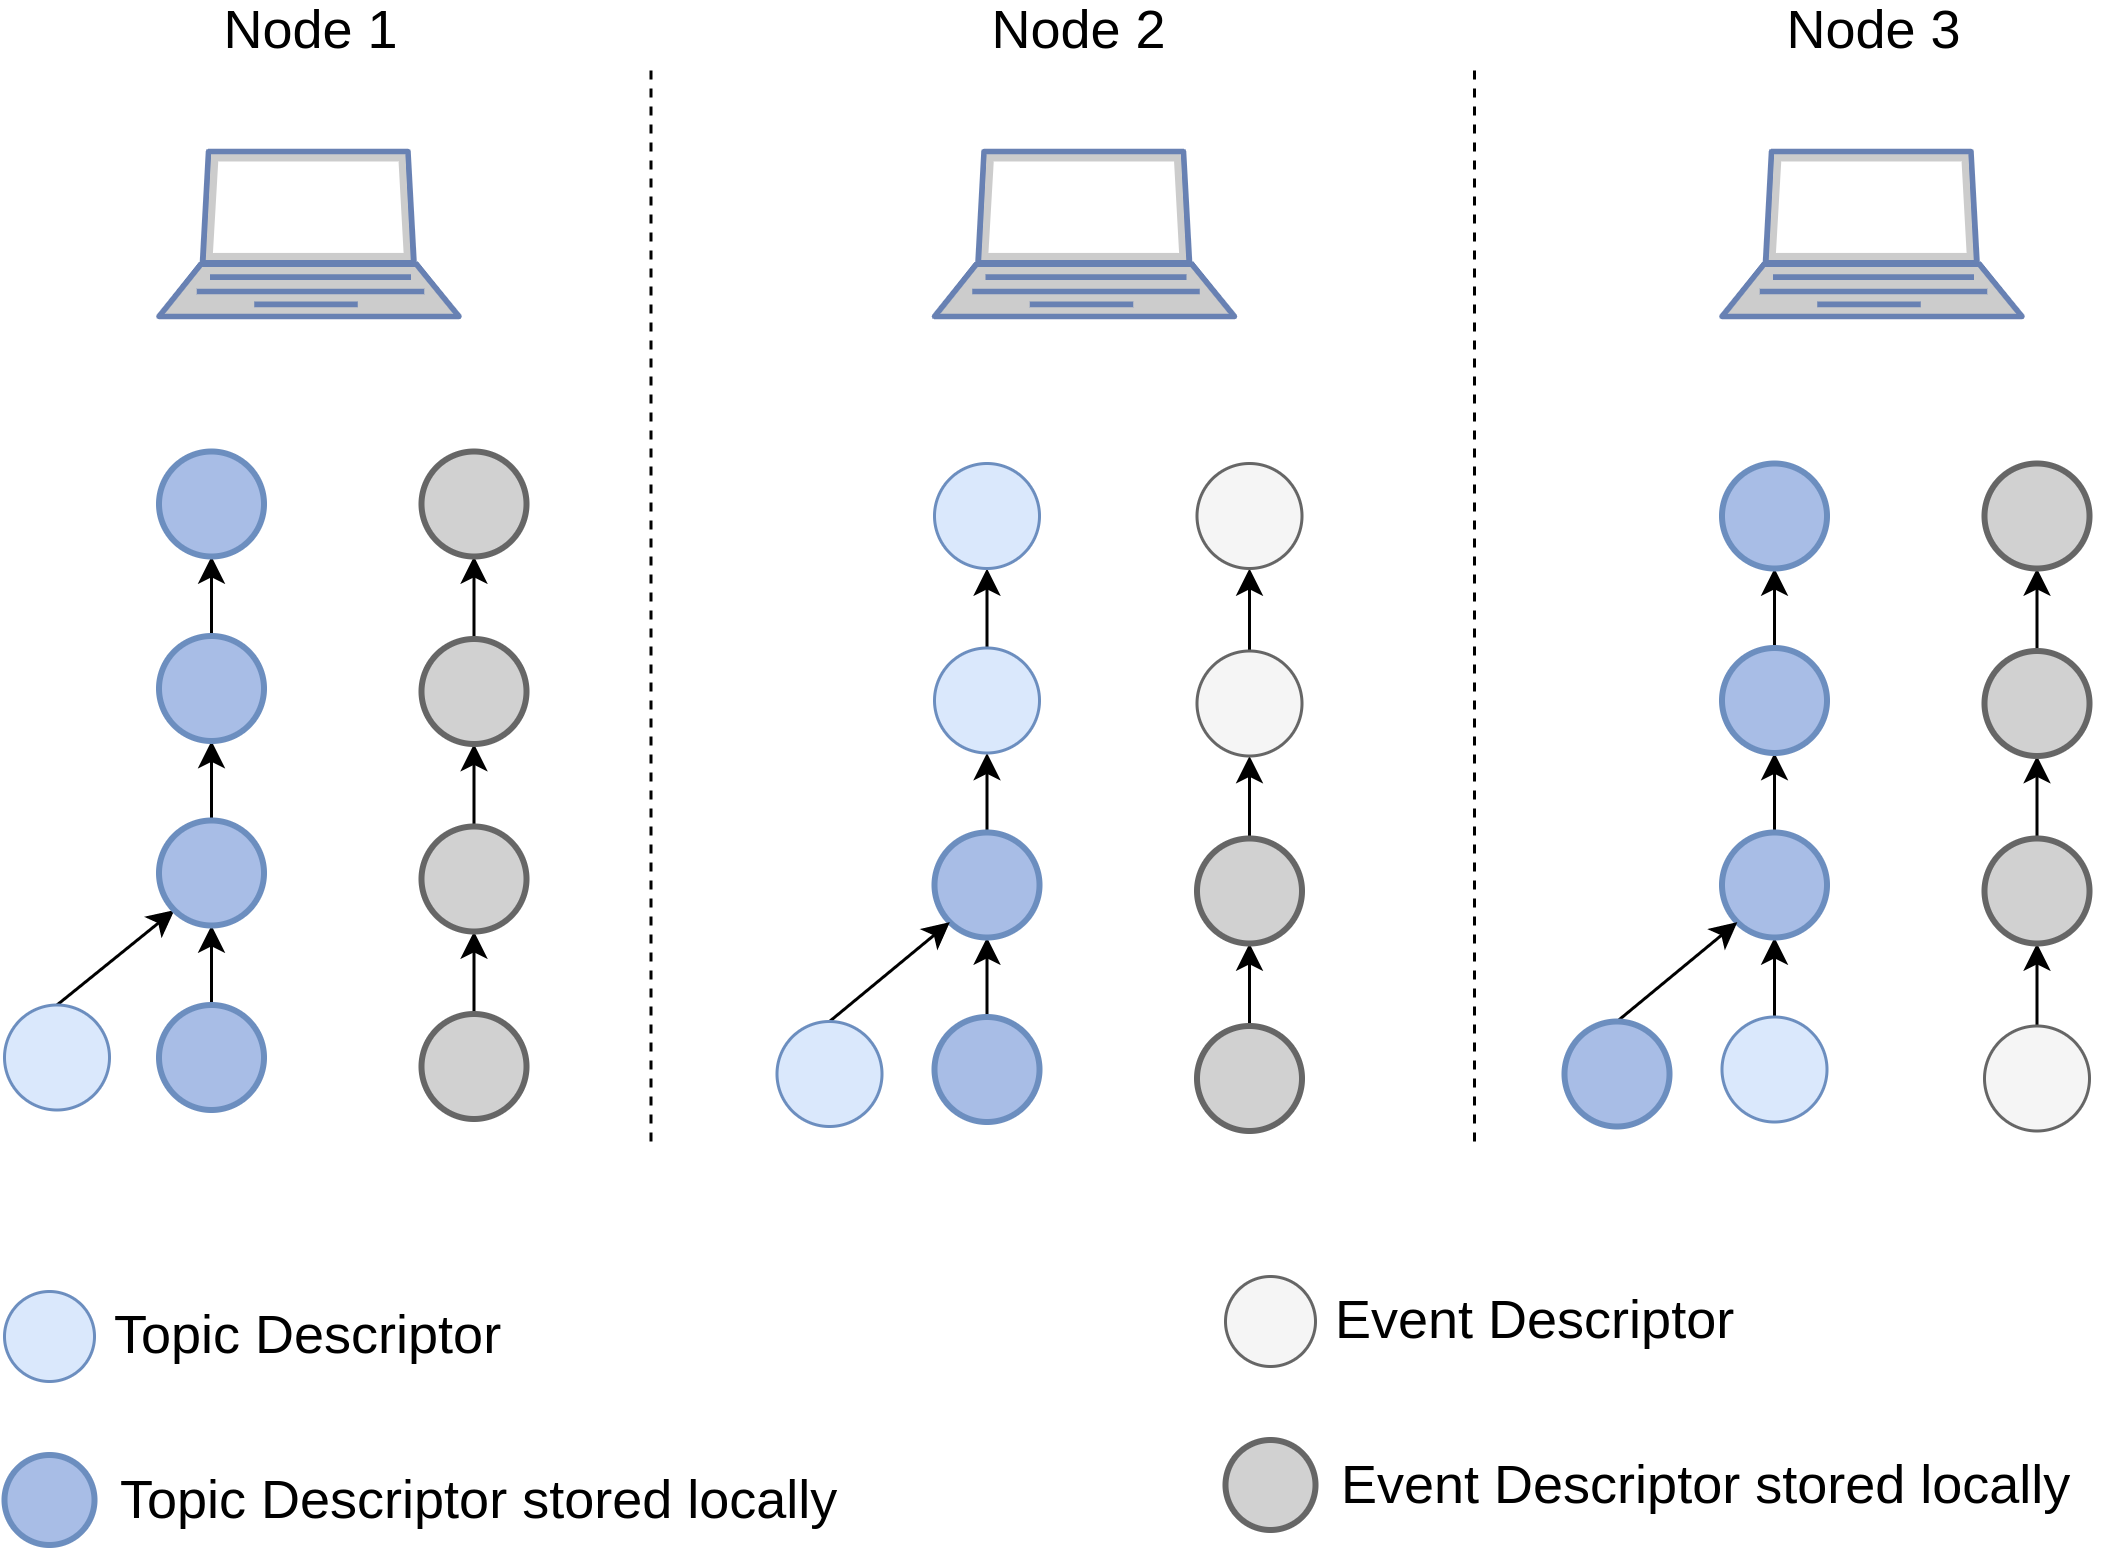
\includegraphics[width=0.8\textwidth]{img/pulsarcast-local-vs-distributed-state.png}
  \caption{Overview of how state is kept across the network}
  \label{fig:pulsarcast-local-vs-distributed-state}
\end{figure}

\section{Subscription Management and Event Dissemination}\label{subscription-management-event-dissemination}

In Pulsarcast, both the subscription management and the event dissemination lie
on top of the multiple overlays built on a per topic basis or, as we call it,
the dissemination trees. These trees represent the path traversed by the events
in order to reach the necessary subscribers, so, in the end, these end up being
the actual representation of both subscriptions and dissemination paths. In
order to better understand them we will start by understanding how the system
handles the creation of topics, new subscriptions, followed by how events are
propagated (with a detailed view of the algorithms used). We will see some of
the configurations the topic descriptor allows for that will change the way
events are propagated and published. Finally, we will run through the messages
sent by each node in order to perform these operations, a crucial part in our
distributed system.

\subsection{Topic creation}\label{subsec:topic-creation}

Before we can speak about a new subscription, a topic must already exist. In
order for this to happen a node starts by creating the meta topic descriptor.
This meta topic descriptor is to be used to disseminate any changes relative to
the topic descriptor at hand and is linked as a sub-topic of it. Procedure
wise, the meta topic is created just like any other topic, with the same
properties (except for its own meta topic of course). Only after it has been
created and stored in the Kadmelia \acrshort{dht} does the node proceed to
create the actual topic descriptor (with the meta topic linked as a sub-topic),
which is then also persisted in the \acrshort{dht}. When any change to the
original topic descriptor is in order, the node creates a new topic descriptor
(remember the immutability of our data structures) but with the original topic
descriptor linked as a parent and with the same meta topic linked as sub-topic.
When these changes happen,  the node publishes the new topic as an event in the
meta topic.  Algorithm \ref{alg:new-topic} provides an overview of the
procedure to create a new topic.

\SetKwProg{Fn}{Function}{}{}

\vspace{8pt}
\begin{algorithm}[H]
  \SetAlgoLined
  \Fn{CreateTopic(newTopic)}{
  	\KwIn{$newTopic=$ data for new topic creation}
		\BlankLine
  	\Begin{
			$parent \leftarrow newTopic.parent$\;
  	  \eIf(\tcp*[r]{Check if the topic has a parent link}){$parent == null$}{
				$metaTopic \leftarrow CreateMetaTopicDescriptor(newTopic)$\;
  	  }{
				$metaTopic \leftarrow parent.subTopics.meta$\;
			}
			$topicData \leftarrow CreateTopicDescriptor(newTopic, metaTopic)$\;
			$Subscribe(metaTopic)$\;
			$Subscribe(topicData)$\;
			$StoreInDHT(metaTopic)$\;
			$StoreInDHT(topicData)$\;
			$Publish(metaTopic, topicData)$\tcp*[r]{Publish the new topic in the meta topic}\
  	}
	}
  \caption{Create a new topic}
	\label{alg:new-topic}
\end{algorithm}
\vspace{8pt}

\subsection{Subscribing}\label{subsec:subscribing}

With the topic descriptor stored and available to the whole network, its
creator will act as the root node in this newly created topic dissemination
tree. When a node wants to subscribe to this topic, it starts by fetching its
descriptor from the Kademlia \acrshort{dht}. After some sanity checks, such as
checking if the node is already part of the dissemination tree, we use the
Kadmelia \acrshort{dht} to find the closest known peer to the author of the
topic. Keep in mind that we are not hitting the network and performing a
Kadmelia lookup operation, we are resorting to information previously stored
locally by the \acrshort{dht} in its K buckets.  The node stores the closest
known peer as its parent in this topic dissemination tree. The join request is
then forwarded to it where the sender peer \acrshort{id} is extracted and used
as its child in this topic dissemination tree, followed by repeating the whole
process. This recursive operation, across multiple nodes in the network, ends
when the join request hits a node that is either already part of the
dissemination tree for this topic or, the actual author of the topic. Algorithm
\ref{alg:subscribe} provides a more detailed generic procedure to be used at
every node when receiving or sending a subscription request (or a join request
as we call it) and Figure \ref{fig:pulsarcast-subscription-flow} tries to
provide a visual representation of the whole subscription flow. In order to
maintain the dissemination trees, every node must keep some state of its
neighbours for every topic. If by some chance a node is unable to connect to a
neighbour, a retry mechanism is in place for a limited amount of retries (a
configurable parameter). If the node is still unable to connect, then it goes
through the subscription procedure again.

\vspace{8pt}
\begin{algorithm}[H]
  \SetAlgoLined
  \Fn{ReceivedJoin(fromNodeId, topicId)}{
      \KwData{$nodeId=$ node id of this node}
      \KwIn{$topicId=$ topic id}
      \KwIn{$fromNodeId=$ node who we got the join request from}
        \BlankLine
      \Begin{
        $topicData \leftarrow GetTopicData(topicId)$\;
        \eIf{$fromNodeId \neq nodeId$}{
        $AddToChildren(t, fromNodeId)$\tcp*[r]{Add as child in dissemination tree}\
                \If(\tcp*[r]{This node is author of the topic}){$topicData.author == nodeId$}{
                    \Return
                }
                \If(\tcp*[r]{Already part of dissemination tree}){$GetParents(topicId) \neq null$}{
                    \Return
                }
        }{
                \If(\tcp*[r]{This node is author of the topic}){$topicData.author == nodeId$}{
                    \Return
                }
            }
        $peer \leftarrow GetClosestKnownPeer(topicData.author)$\;
      $AddToParents(topicData.id, peer)$\tcp*[r]{Add as parent in dissemination tree}\
            $SendRPC(topicData.id, peer)$\;
      }
    }
  \caption{Join request handler for each node}
    \label{alg:subscribe}
\end{algorithm}
\vspace{8pt}

\begin{figure}[hb!]
  \centering
  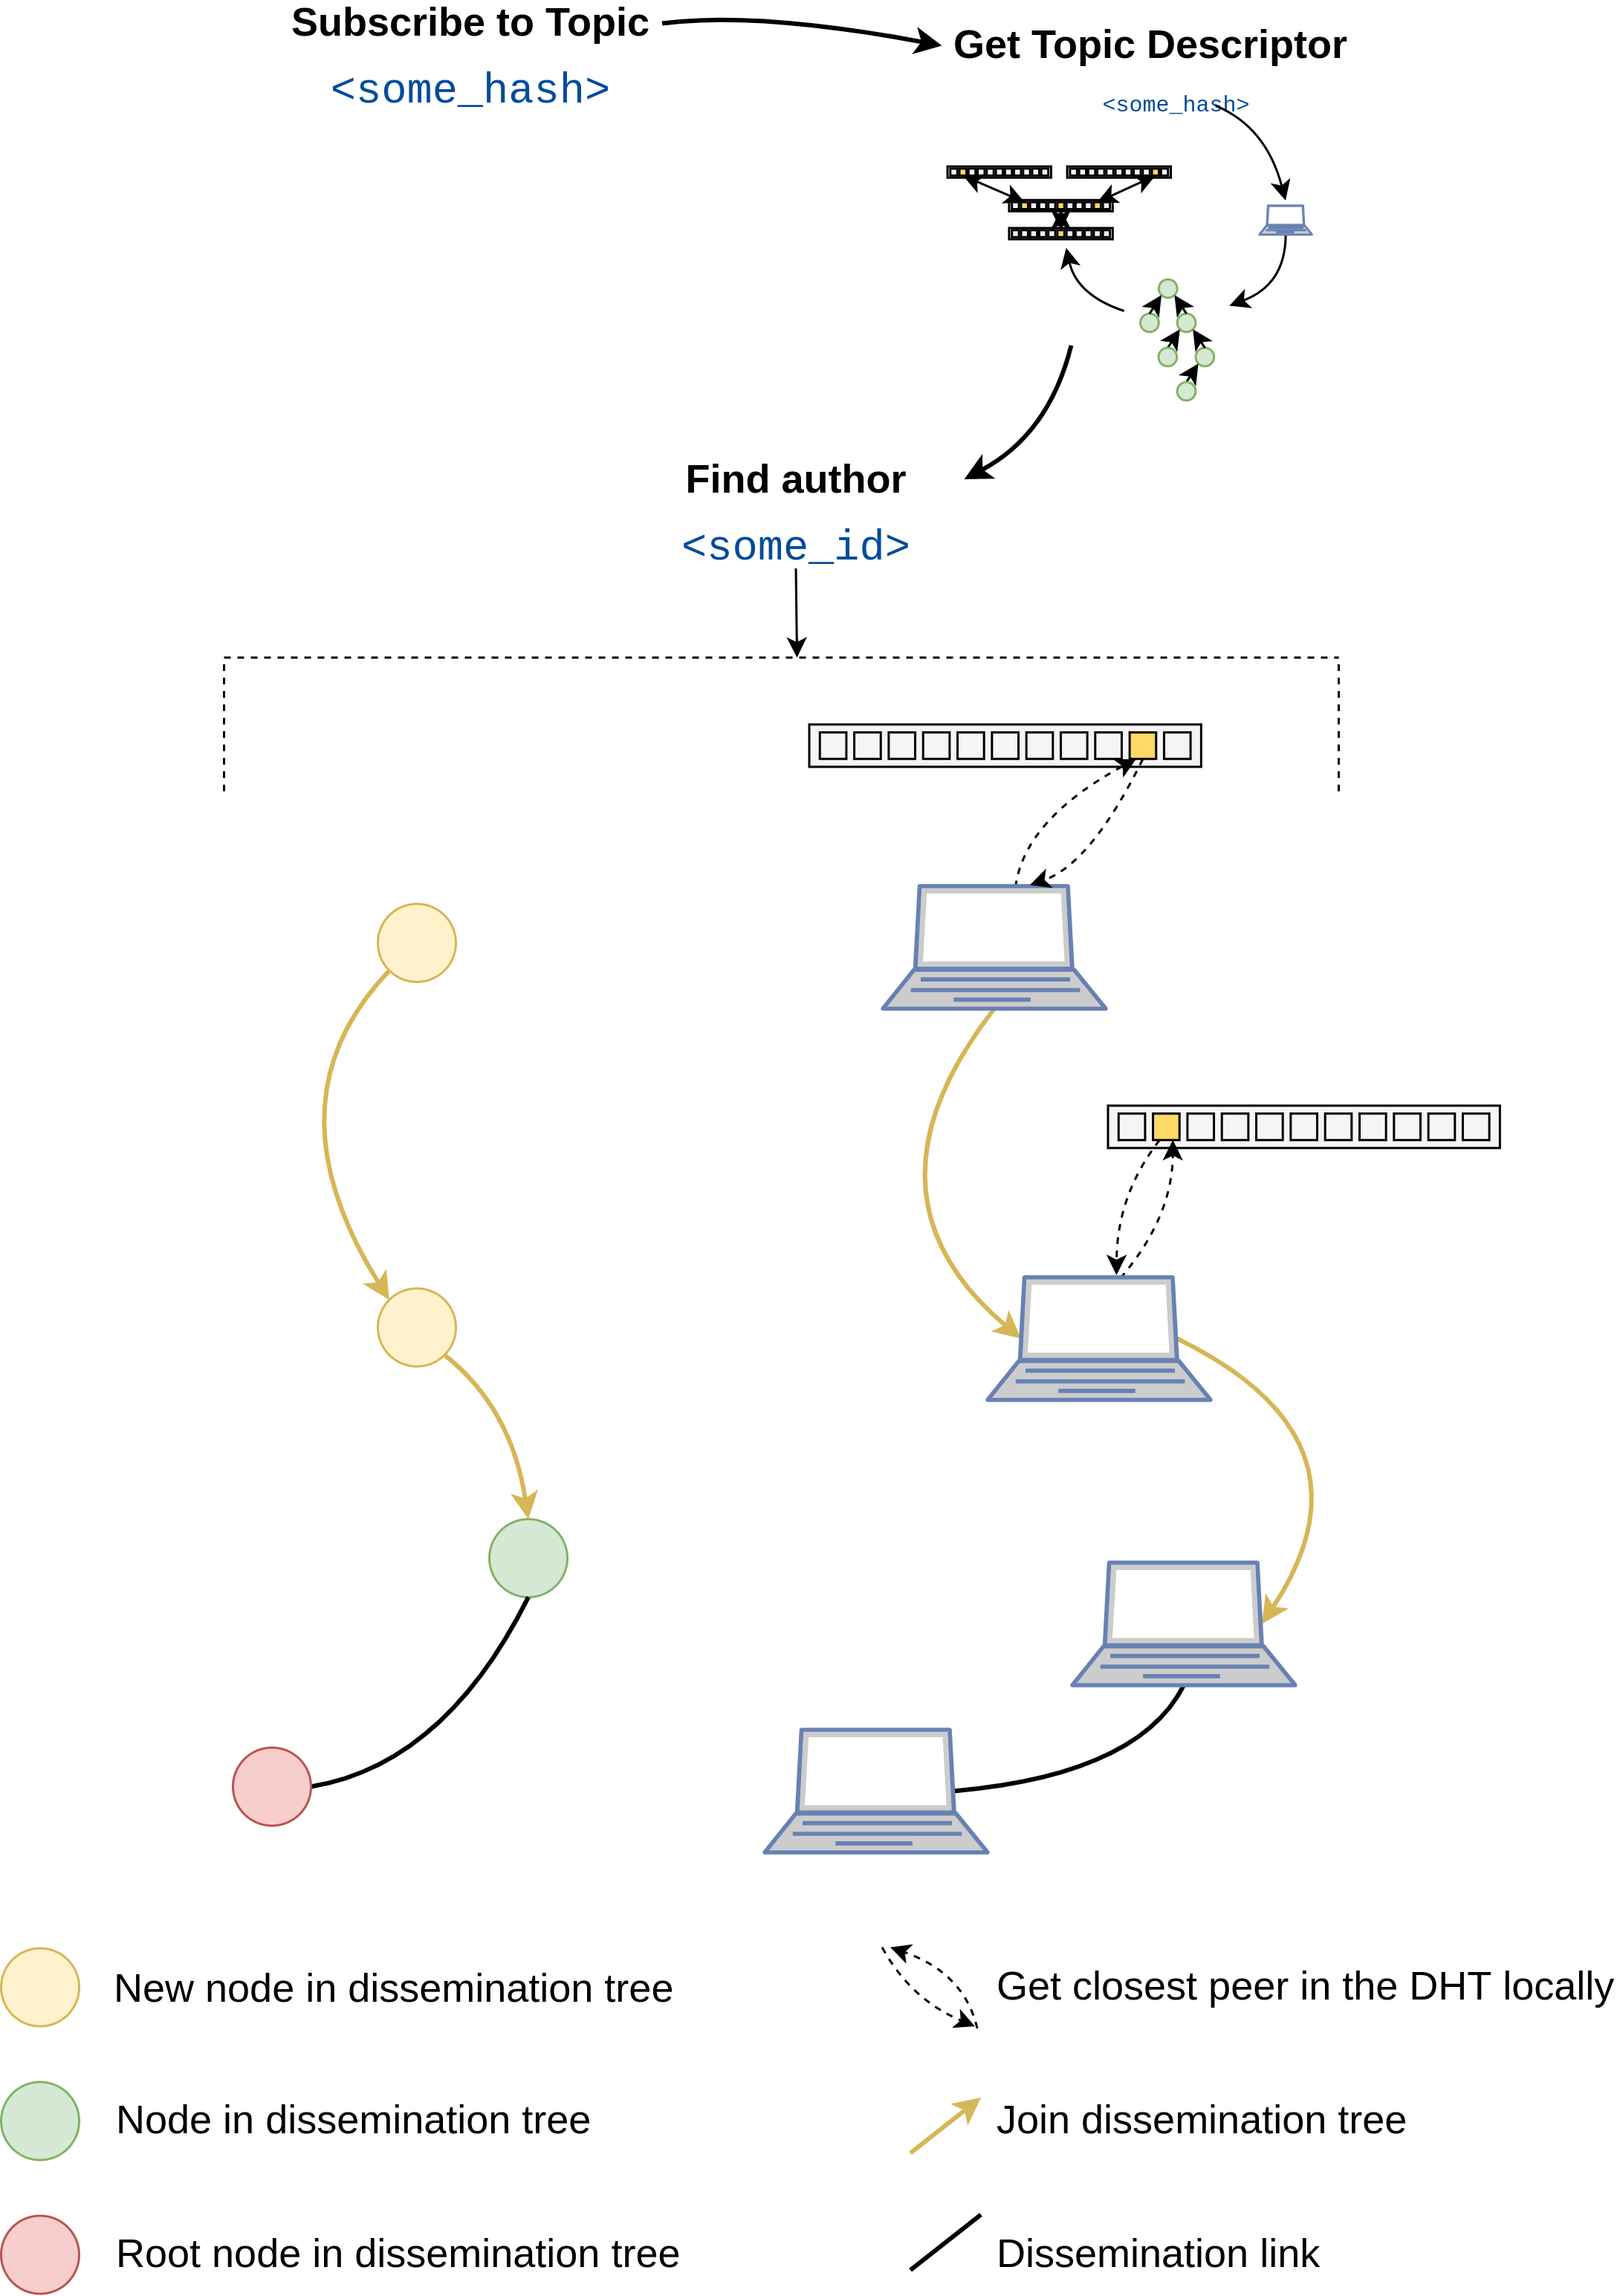
\includegraphics[width=0.8\textwidth]{img/pulsarcast-subscription-flow.png}
  \caption{Overview of the flow for creating a new subscription}
  \label{fig:pulsarcast-subscription-flow}
\end{figure}

\subsection{Publishing and event dissemination}\label{subsec:publishing-and-event-dissemination}

Considering the topic creation and subscription management previously discussed
we can see that event dissemination becomes easier to handle, almost as a
consequence of the way the subscription management is built, and dissemination
trees again play their key part here. Pulsarcast, however, allows for some
additional customisation and configuration at the topic level focused on
providing a lot more flexibility to our system. When a node is creating a
topic, it can configure:
\begin{itemize}
  \item
    Which nodes are allowed to publish
  \item
     If and which nodes can request to publish
  \item
    How events are linked together (through the parent link)
\end{itemize}

These options are \emph{requestToPublish}, \emph{allowedPublishers} and
\emph{eventLinking}, mentioned previously in Section \ref{data-structures},
we will see how each one of these fits together with the way Pulsarcast nodes
dissminate events. Figures \ref{fig:pulsarcast-publish-order-guarantee} and
\ref{fig:pulsarcast-publish-custom} provide visual aids to how these options
come together for event dissemination.

\begin{figure}[hb!]
  \centering
  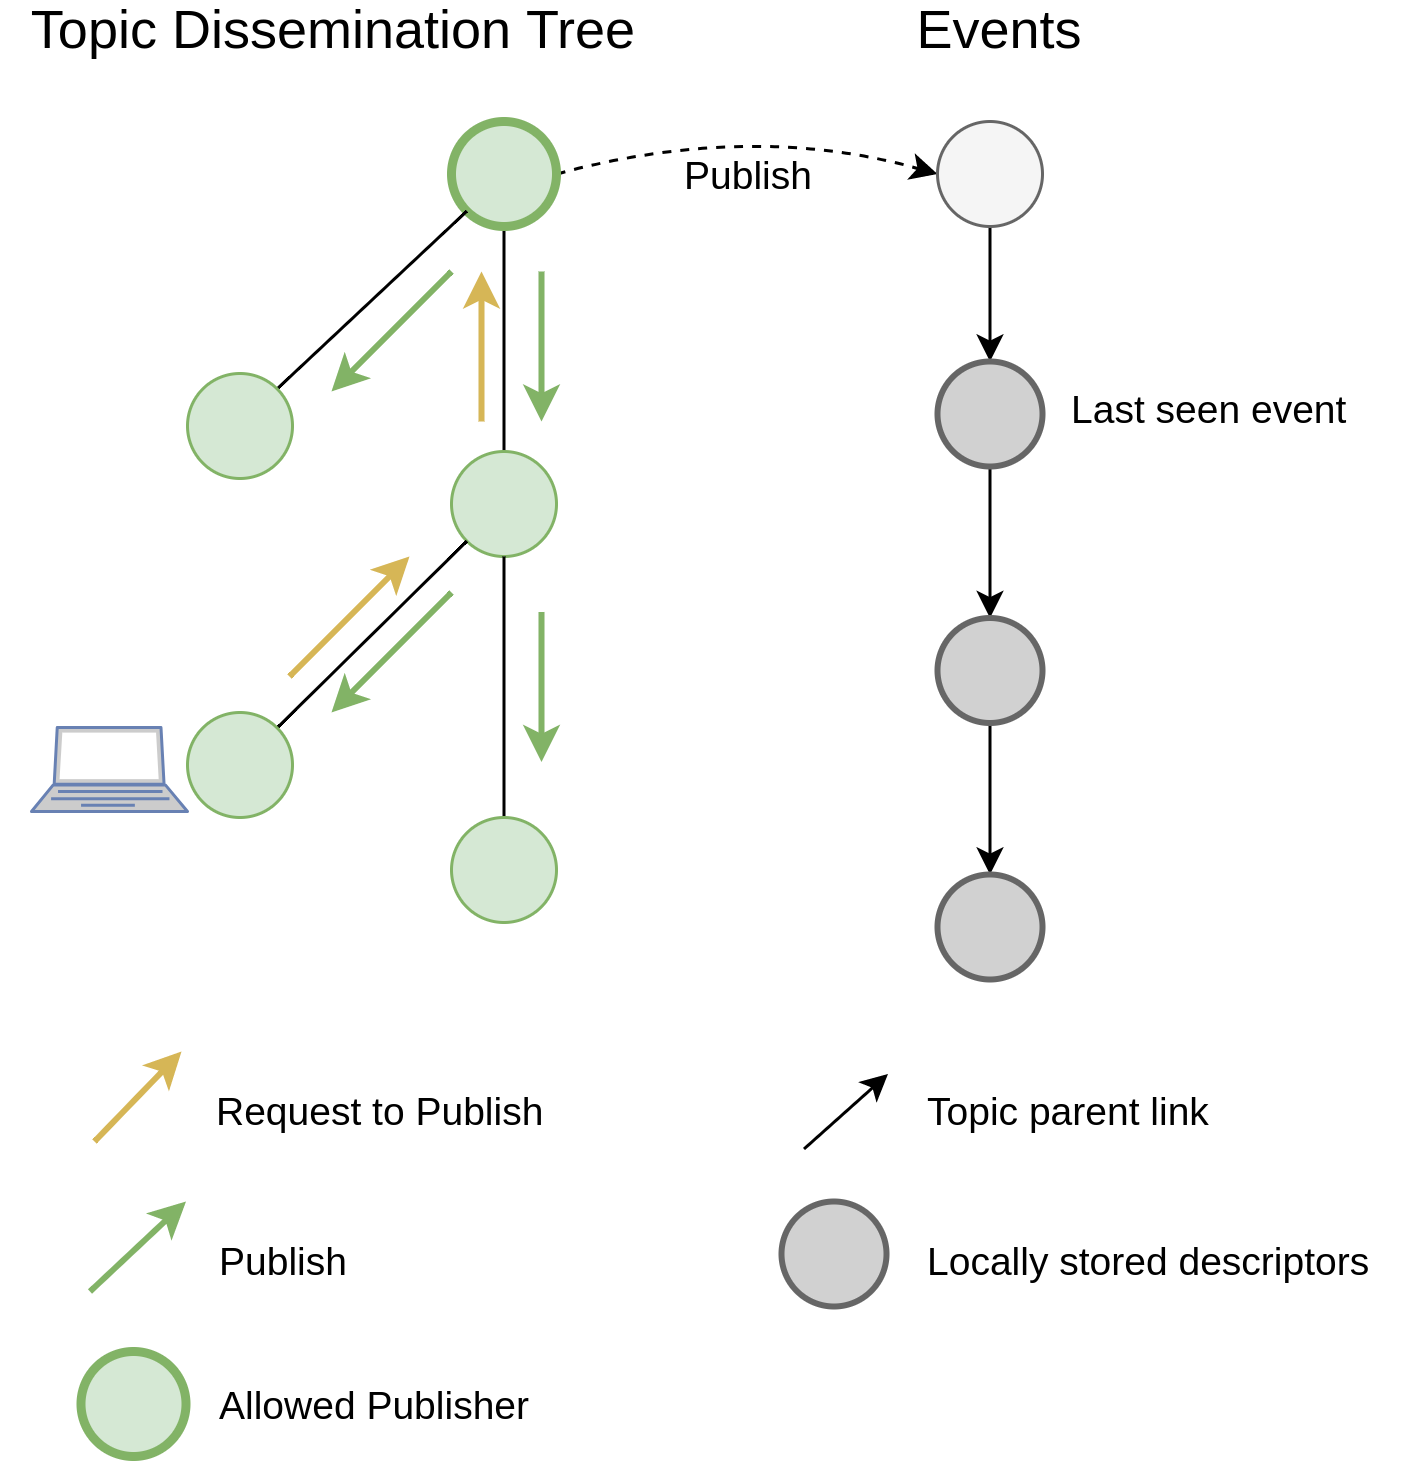
\includegraphics[width=0.6\textwidth]{img/pulsarcast-publish-order-guarantee.png}
  \caption{Event dissemination mechanism for a topic with only the author allowed to publish, last seen event linking and request to publish allowed. This scenario provides order guarantee.}
  \label{fig:pulsarcast-publish-order-guarantee}
\end{figure}

\begin{figure}[hb!]
  \centering
  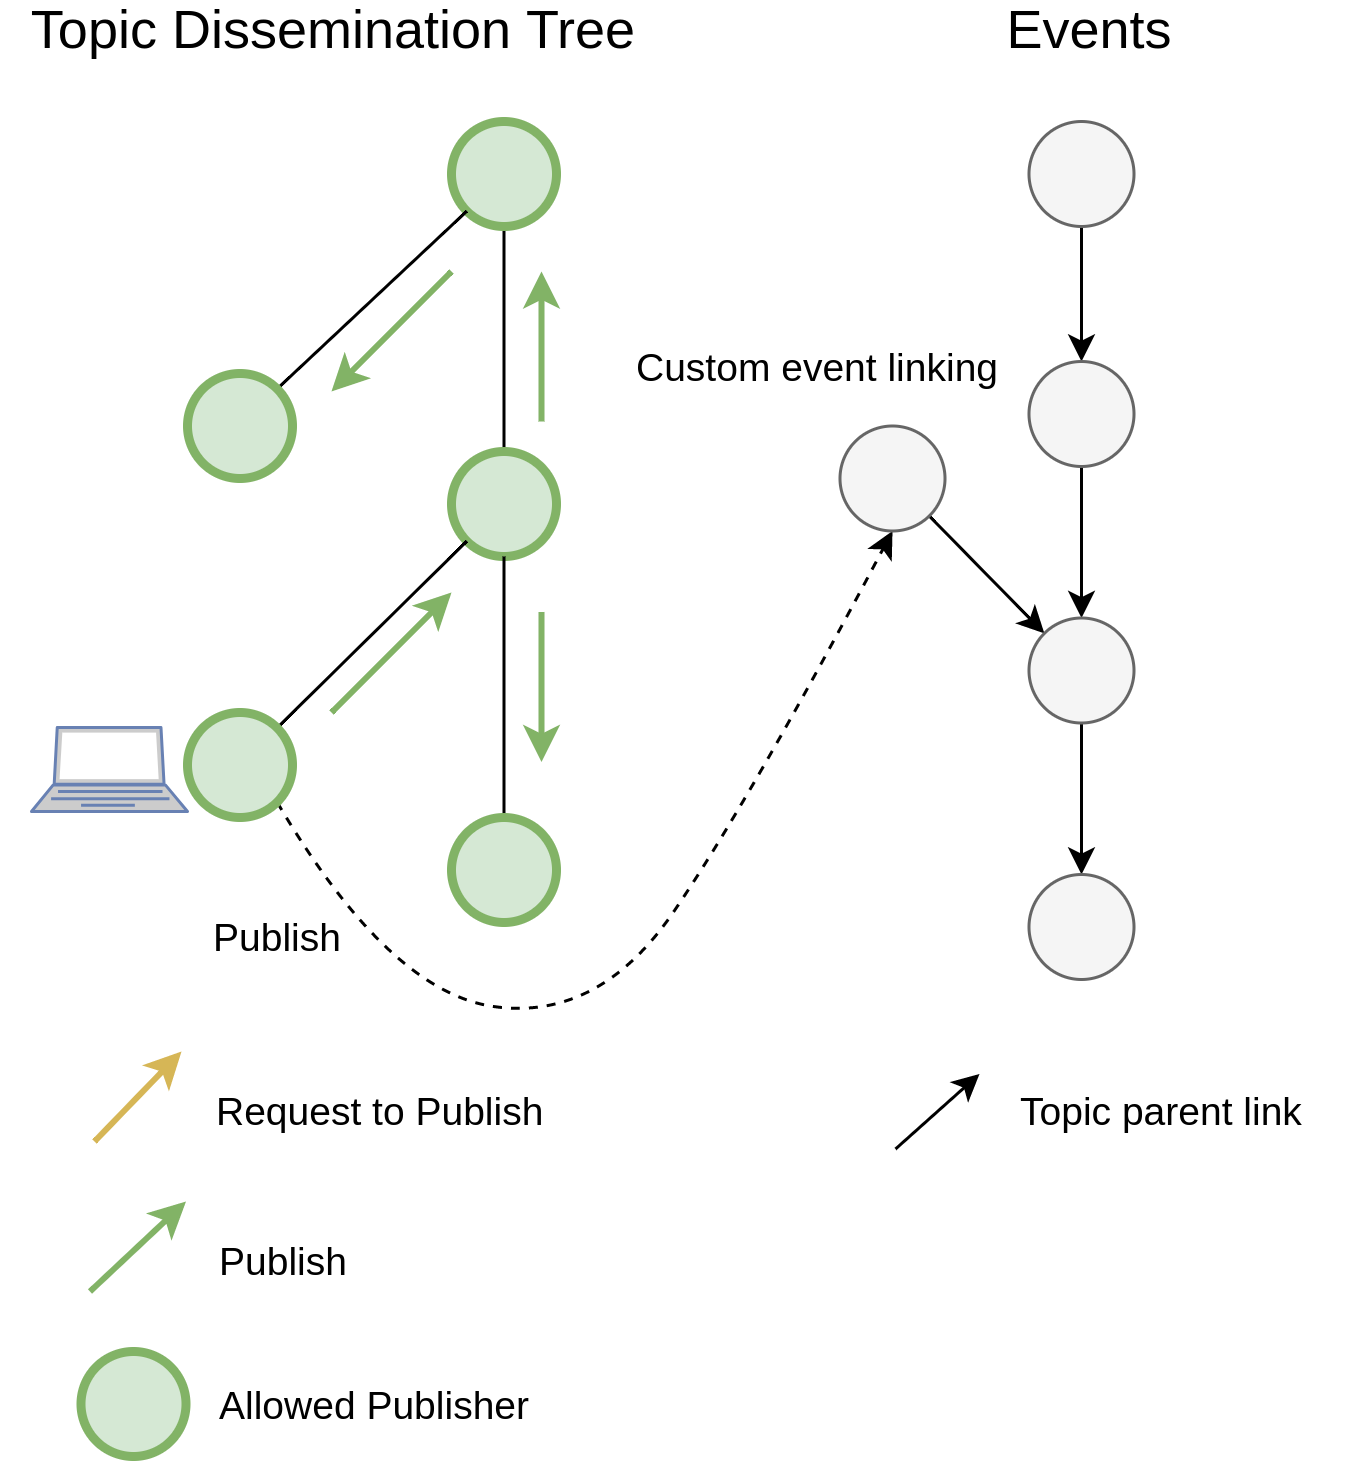
\includegraphics[width=0.6\textwidth]{img/pulsarcast-publish-custom.png}
  \caption{Event dissemination mechanism for a topic with custom event linking and global publishers allowed}
  \label{fig:pulsarcast-publish-custom}
\end{figure}

When a node wants to publish an event in a topic, it starts by fetching the
topic descriptor, first locally and then, if it is not present, from the
Kadmelia \acrshort{dht}.  This way, we have access to the topic data as well as its
configurations. The node then checks if it is allowed to publish through the
topic configuration whitelist mechanism. This option, \emph{allowedPublishers},
can either be enabled and, if so, a list of nodes is provided that is checked
before publishing, or it can be disabled, and in that scenario, every node can
publish a message. If the node cannot publish the message, it will check if it
can submit a request to publish. This request to publish is another option set
in the topic descriptor, through the \emph{requestToPublish} field, that, if
enabled, allows every node in the network to submit these special requests.
Optionally, it can also be a whitelist of nodes allowed to submit these. When a
node forwards a request to publish across the network, it propagates across the
dissemination tree (from children nodes to parents) until it eventually finds a
node which is allowed to publish this event. This will dictate the difference
in the publisher (node who actually publishes the content) and the author (node
responsible for creating the content in the first place).

Upon receiving a publish event request, whether if it was initiated at this
node or through a remote request to publish, the node starts by appropriately
linking the new event to a parent event. This is where the \emph{eventLinking}
option in our topic descriptor comes into play. Right now this option can
either be \emph{CUSTOM} or \emph{LAST\_SEEN}. When the topic allows for custom
linking, the client application can set a custom parent event, as long as it
exists. With the last seen option, however, the Pulsarcast node takes care of
linking the given event to the event last seen by it. After the linking is
done, the node can safely store the event descriptor in the Kademlia \acrshort{dht},
followed by disseminating it through its children and parent nodes in this
topic dissemination tree. From this point forward, nodes along the
dissemination tree will forward the event across branches of the tree where
this has not gone through. All of the logic we have covered around event
dissemination is better detailed in the Algorithms \ref{alg:receive-event} and
\ref{alg:send-event}.

\vspace{8pt}
\begin{algorithm}[H]
  \SetAlgoLined
  \Fn{ReceivedEvent(fromNodeId, eventData)}{
      \KwData{$nodeId=$ node id of this node}
      \KwIn{$fromNodeId=$ node who we got the event from}
      \KwIn{$eventData=$ event descriptor}
        \BlankLine
      \Begin{
        $topicData \leftarrow GetTopicData(eventData.topicId)$\;
        \eIf{$AllowedToPublish(nodeId, topicData)$}{
                $SendEvent(fromNodeId, eventData)$\;
        }{
                \If{$AllowedToRequestToPublish(nodeId, topicData$}{
                    $SendRequestToPublish(eventData)$\tcp*[r]{Send request to publish to parent node}\
                }
            }
      }
    }
  \caption{Event handler for each node}
    \label{alg:receive-event}
\end{algorithm}
\vspace{8pt}

\vspace{8pt}
\begin{algorithm}[H]
  \SetAlgoLined
  \Fn{SendEvent(eventData)}{
      \KwData{$nodeId=$ node id of this node}
      \KwIn{$fromNodeId=$ node who we got the event from}
      \KwIn{$eventData=$ event descriptor}
        \BlankLine
      \Begin{
        $topicData \leftarrow GetTopicData(eventData.topicId)$\;
            \If{$IsNewEvent(eventData)$} {
                $linkedEvent \leftarrow LinkEvent(eventData)$\tcp*[r]{Add parent link}\
                $StoreInDHT(linkedEvent)$\;
            }
            \If{$(IsSubscribed(eventData.topicId)==true)$} {
                $EmitEvent(eventData.topicId, eventData)$\;
            }
            \For{$peer \leftarrow GetChildren(eventData.topicId), GetParents(eventData.topicId)$}{
                \If(\tcp*[r]{Do not send the event back}){$fromNodeId \neq peer$}{
                    $SendRPC(eventData, peer)$\;
                }
            }
      }
    }
  \caption{Event forwarding function}
    \label{alg:send-event}
\end{algorithm}
\vspace{8pt}

It is essential to understand some of the properties that these multiple
configuration options allow. The simplest example would be a scenario where
only the author of a topic is allowed to publish, event linking is based on the
last seen event and request to publish is allowed. In this example, despite
every node being allowed to create content, we can achieve order guarantee,
with a single stream of events all linked together. Another example would be a
scenario where we have a whitelist of allowed publishers, no request to publish
allowed and last seen event linking taking place. With this, we get a simple
producer/consumer scenario, with a list of a few selected and vouched for
producers that every node is aware of (that could even be expanded later on by
the topic author). Finally, on the other end of the spectrum, we have a
scenario where everyone is allowed to publish, and custom event linking is
allowed. Here, we are essentially giving the ability for clients and
applications to use event trees to represent data in however they see fit given
that, with custom event linking, applications can shape the event trees however
they like. Links can go as far as to imply event causality if applications are
programmed and configured as such. All of these scenarios came from a
realisation that it did not make sense to limit Pulsarcast's uses out of the
box, especially taking account that through simple configuration we could cater
for a broader set of use cases and applications.

\section{\acrshort{rpc} message protocol}\label{rpc-message}

We have run through the overall architecture of Pulsarcast. However, we still
have not detailed how the nodes communicate with each other. The fact is,
Pulsarcast does not favour or define the usage of a specific wire protocol. In
our view Pulsarcast can and should work independently of what we use in the
transport layer. It does, however, specify a well-defined communication
protocol built using Protocol
Buffers~\footnote{\url{https://developers.google.com/protocol-buffers/}}. Protocol
Buffers (or protobuf for short) are Google's open-source, language-neutral,
platform-neutral, extensible mechanism for serializing structured data. It
allows us to define common lightweight interfaces that, through source code
generation, work across platforms. Plus, it is fast and quite small once
encoded to the protocol buffer binary format (what actually runs in the wire),
while also supporting a text-based representation, similar to JSON, for
readability purposes. With protobuf's, we have defined a set of \acrfull{rpc}
schemas used by our system to communicate between nodes.

We started by defining a common interface for all of our \acrshort{rpc}
messages as showed in Listing \ref{proto-rpc-message}. In protobufs, every
field is associated with a number. These are used to identify a field in the
protobuf binary
format~\footnote{\url{https://developers.google.com/protocol-buffers/docs/encoding}}
uniquely.  Our message format is quite straightforward, with three fields,
\emph{op} (for operation), \emph{payload} representing a generic payload and
finally \emph{metadata} containing relevant metadata such as the creation date
of this message and the protocol version used. The supported operations for now
essentially translate all the actions a node might undertake, which are
publishing an event, joining a topic, leaving a topic, creating a topic and
requesting to publish. The payload is an abstraction, and it can hold a topic
descriptor, an event descriptor or a topic \acrshort{id} depending on the
operation field of this message. Finally, the \acrshort{rpc} schema itself is
an array of the messages, so that if needed a node can forward multiple
operations in one go.

% \noindent\begin{minipage}{\textwidth}
% \vspace{8pt}
\begin{lstlisting}[float, language=protobuf3,caption={Protobuf schema for our
\acrshort{rpc} messages},label={proto-rpc-message}]
message RPC {
  enum Operation {
    PUBLISH_EVENT = 2;
    JOIN_TOPIC = 3;
    LEAVE_TOPIC = 4;
    NEW_TOPIC = 5;
    REQUEST_TO_PUBLISH = 6;
  }

  message Message {
    optional Operation op = 1;
    oneof payload {
      TopicDescriptor topic = 2;
      EventDescriptor event = 3;
      bytes topicId = 5;
    }
    optional MetaData metadata = 6;
  }

  message MetaData {
    optional string created = 1;
    optional string protocolVersion = 2;
  }

  repeated Message msgs = 1;
}
\end{lstlisting}
% \vspace{8pt}
% \end{minipage}

The topic and event descriptors also have a specific protobuf schema,
essentially a representation of what we have already covered in Section
\ref{data-structures}. Listings \ref{proto-topic-descriptor} and
\ref{proto-event-descriptor} show us the specification of these. In order to
keep our messages as lightweight as possible and avoid unnecessarily burdening
the network, we opted to have all of our content identifiers (such as the
author and links) sent in binary format. Otherwise, the remaining fields end up
being a one to one mapping from the data structure schemas of the event
descriptor and topic descriptor.

% \noindent\begin{minipage}{\textwidth}
% \vspace{8pt}
\begin{lstlisting}[float, language=protobuf3,caption={Protobuf schema of the topic descriptor},label={proto-topic-descriptor}]
message Link {
  optional bytes / = 1;
}

message TopicDescriptor {

  optional string name = 1;
  optional bytes author = 2;
  optional Link parent = 2;
  map<string, Link> # = 3;
  optional MetaData metadata = 4;

  message MetaData {

    enum EventLinking {
      LAST_SEEN = 0;
      CUSTOM = 1;
    }

    message PublishersList {
      optional bool enabled = 1;
      repeated bytes publishers = 2;
    }

    optional string created = 1;
    optional string protocolVersion = 2;
    optional PublishersList allowedPublishers = 3;
    optional PublishersList requestToPublish = 4;
    optional EventLinking eventLinking = 5;
  }
}
\end{lstlisting}
% \vspace{8pt}
% \end{minipage}

% \noindent\begin{minipage}{\textwidth}
% \vspace{8pt}
\begin{lstlisting}[float, language=protobuf3,caption={Protobuf schema of the event descriptor},label={proto-event-descriptor}]
message Link {
  optional bytes / = 1;
}

message EventDescriptor {

  message MetaData {
    optional string created = 1;
    optional string protocolVersion = 2;
  }

  optional bytes author = 1;
  optional Link topic = 2;
  optional bytes payload = 3;
  optional bytes publisher = 4;
  optional Link parent = 5;
  optional MetaData metadata = 6;
}
\end{lstlisting}
% \vspace{8pt}
% \end{minipage}

\section{Summary}\label{summary}

In this chapter, we presented a technical and architectural overview of
Pulsarcast. We started by introducing the use case for our decentralised
topic-based system in Section \ref{use-case}, with a brief overview of what we
are seeking to accomplish as well as our broader architectural decisions. We
looked at how clients can interact with our system (create a topic, publish,
subscribe and unsubscribe) and how the Kadmelia \acrshort{dht} powers our
underlying system and its dissemination trees.

In Section \ref{data-structures}, we introduced our immutable,
content-addressable data structures, based on the Merkle \acrshort{dag},
representing events and topics and how these are distributed across the
network.

Applying the taxonomy we had previously defined in Chapter
\ref{chapter:related-work}, we looked into how subscriptions are managed and
events are disseminated in Section
\ref{subscription-management-event-dissemination}, focusing on the algorithms
responsible for topic creation, subscription handling and event handling.

Finally, we focused on how Pulsarcast works under the hood in Section
\ref{rpc-message}, taking a closer look at how our \acrshort{rpc} messages,
built using Protocol Buffer, drive all the functionality we described
previously.

